This chapter is in preparation to be submitted to the astronomical literature, with working author list Kate Storey-Fisher, David W. Hogg, Hans-Walter Rix, Anna-Christina Eilers, and Giulio Fabbian.

\graphicspath{{figures/figures_quaia/}}


\section{Chapter Abstract}
\Gaia DR3 contains \val{N_gall} sources that are classified as possible quasars, with estimated redshifts from low-resolution BP/RP spectra.
These quasar candidates comprise an unprecedented resource for extragalactic and large-scale structure science: they are all-sky and have a median redshift of $z \sim \val{z_med_gall}$, hence covering more comoving volume than any other quasar sample.
While the quasar candidate catalog is highly complete, it has low purity.
Further, $\val{p_outliers_gall_zgaia_dzhi_Glo}\%$ of quasar candidates with $G<\Glo$ have highly inaccurate redshift estimates ($|\dz| > \val{dzhi}$) when compared to redshifts obtained by the Sloan Digital Sky Survey (\SDSS).
In this work, we construct a quasar catalog based on the \Gaia candidates sample as well as unWISE infrared observations (based on the Wide-Field Infrared Survey Explorer survey) that is suitable for cosmological and other analyses.
To decontaminate the sample, we apply cuts based on proper motions and \Gaia and unWISE colors, reducing the number of contaminants by an estimated \val{factor_reduction_contaminants}.
We improve the redshifts by training a $k$-nearest neighbors model based on colors and \Gaia redshift estimates with \SDSS redshift labels, and achieve a sample with only $\val{p_outliers_zspz_dzhi_Glo}\%$ ($\val{p_outliers_zspz_dzmid_Glo}\%$) catastrophic redshift errors with $|\dz| > \val{dzhi}$ ($\val{dzmid}$) on our spectro-photometric redshift estimates, a reduction of \val{factor_reduction_outliers_dzhi_Glo} (\val{factor_reduction_outliers_dzmid_Glo}) compared to the \Gaia redshifts.
The final catalog, the \catalog (\cat), has \val{N_gcathi} quasar candidates with a $G<\Ghi$, and \val{N_gcatlo} candidates in the even cleaner $G<\Glo$ sample.
We construct a rigorous all-sky selection function model for the sample, incorporating dust extinction, stellar source crowding, and the \Gaia scanning law. 
We verify our catalog against other quasar catalogs, and describe possible applications and limitations.
The catalog is publicly available \texttt{here}. 


\section{Introduction}

Quasars are powerful tools for many fields of astrophysics. 
They are key probes of accretion physics (e.g. \citealt{SunyaevZeldovich1970, yu_quasar_2020}), which informs the evolution of active galactic nuclei (AGN). 
The evolution of quasars and their host galaxies are intertwined, giving insight into supermassive black hole growth (e.g. \citealt{hopkins_unified_2006}) as well as massive galaxy formation (e.g. \citealt{kormendy_coevolution_2013}).
Studies of the quasar distribution can also be used to understand black hole evolution (e.g. \citealt{powell_clustering_2020}) and halo masses and environmental effects (e.g. \citealt{dipompeo_characteristic_2017}).
Quasars are  key background sources for other cosmic phenomena such as gravitational lenses (e.g. \citealt{claeskens_gravitational_2002}), and quasar spectra encode the properties of the intergalactic medium via the Lyman alpha forest (e.g. \citealt{rauch_lyman_1998}). 

Quasars are key tracers for large-scale structure cosmology.
They reside in peaks of the dark matter distribution and their clustering can be used to measure cosmological parameters, including the baryon density $\Omega_b$, the cosmological constant $\Omega_\Lambda$, the Hubble distance $D_H$, and the growth rate of structure $f\sigma_8$ (e.g. \citealt{yahata_large-scale_2005, hou_completed_2020}).
Cross-correlations between quasars and other tracers provide measurements of key quantities, such as with photometric galaxy samples to measure the baryon acoustic feature (e.g. \citealt{}), with cosmic microwave background lensing to constrain quasar bias (e.g. \citealt{sherwin_atacama_2012}), and with foreground galaxies as a probe of weak lensing (e.g. \citealt{menard_cosmological_2002, scranton_detection_2005, zarrouk_baryon_2021}).
They can also be used as standardizable candles to measure the expansion rate of the universe (e.g. \citealt{setti_hubble_1973, risaliti_hubble_2015, lusso_quasars_2020}).
Finally, the quasar distribution provides a test of the cosmological principle of isotropy and homogeneity (e.g. \citealt{secrest_test_2021, dam_testing_2022}).

Many surveys have observed and cataloged quasars, with several million currently identified across surveys.
The latest Sloan Digital Sky Survey data release, DR16, includes a highly complete catalog of 750,414 quasars with spectroscopic redshifts \citep{lyke_sloan_2020}.
Photometric surveys observe a much larger number of quasars, at the expense of low redshift accuracy; nearly three million quasars with reliable photometric redshifts have been cataloged \citep{kunsagi-mate_photometric_2022}, including with WISE \citep{wright_wide-field_2010} which imaged the entire sky and PAN-STARRS \citep{chambers_pan-starrs1_2019} which observed three-quarters of the sky.
Upcoming surveys will observe even more quasars: the Dark Energy Spectroscopic Instrument (DESI, \citealt{Aghamousa2016}) expects to obtain spectra for 3 million quasars, and the Rubin Observatory's LSST will photometrically observe upwards of 10 million quasars \citep{ivezic_lsst_2016}.
However, none of these quasar catalogs is both all-sky and contains precise redshift information.
The recently released \Gaia DR3 quasar candidates \citep{gaia_collab_gaia_2022} constitute a new sample that fills this gap. 

The \Gaia quasar catalog presents a new opportunity to explore these science questions.
While the \Gaia satellite was designed to map the stars in the Milky Way \citep{gaia_collaboration_gaia_2016}, it broadly observes bright objects in the sky, which includes many extragalactic sources. 
In DR3, the \Gaia collaboration released a sample of 6,649,162 quasar candidates that were incidentally observed during the survey \citep{gaia_collab_gaia_2022}.
The sources cover the entire sky and have \Gaia BP/RP spectra, low-resolution spectra covering the wavelength range 330-1050 nm. 
These spectra allow for redshift estimates of the sources, with $\val{p_acc_gall_zreliable_zgaia_dzlo}\%$ having a precision of $|\dz| < \val{dzlo}$ compared to \SDSS redshifts when no redshift warning flags are set, which is the case for $\val{p_zreliable_gall}\%$ of the sample (for the full sample, this decreases to $\val{p_acc_gall_zgaia_dzlo}\%$).
While not as precise as high-resolution spectroscopic redshifts, they are significantly better than photometric redshifts. 
The median redshift of the sample is $z=\val{z_med_gall}$. 
The \Gaia quasar candidate sample was constructed for completeness over purity, and has an estimated purity of 52\%; the \Gaia collaboration also suggests criteria for a higher purity ($\sim$95\%) sub-catalog of $\sim$1.9 million quasars.
Overall, the sample presents an unprecedented resource for quasar science and cosmology.

There are two main issues with this raw \Gaia sample.
First, the sample contains a large number of non-quasar contaminants.
Second, a significant fraction of the redshift estimates are catastrophic errors, due to emission line misidentification given the limitations of the spectra.
In this work, we construct a clean quasar catalog with low contamination and improved redshift estimates, with the particular goal of building a catalog appropriate for large-scale structure analyses, as well as other quasar science.
For both of these, we rely on cross-matches with unWISE observations of the quasars, which adds key infrared information.
To filter out contaminants, we apply color cuts based on the \Gaia and WISE photometry, as well as a proper motion cut.
To improve the redshifts, we identify quasars that are also observed by \SDSS for which we have highly precise spectroscopic redshifts, and train a $k$-Nearest-Neighbors ($k$NN) model based on their photometry and \Gaia redshift estimates.
Further, the \Gaia quasar candidates sample has strong systematic imprints from various observational effects, such as galactic dust.
We fit a model for the selection function based on observational templates using a Gaussian process; this map is a key ingredient in many analyses.

This paper is organized as follows.
In \S\ref{sec:data}, we describe the initial data sets used in the construction of the catalog.
The catalog construction is detailed in \S\ref{sec:construction}.
In \S\ref{sec:catalog}, we present the final catalog and perform verification and comparisons to other samples, and outline the data format.
We summarize the catalog and describe data access in \S\ref{sec:summary}.

\section{Initial Data Sets}
\label{sec:data}

\begin{figure}
    \centering
    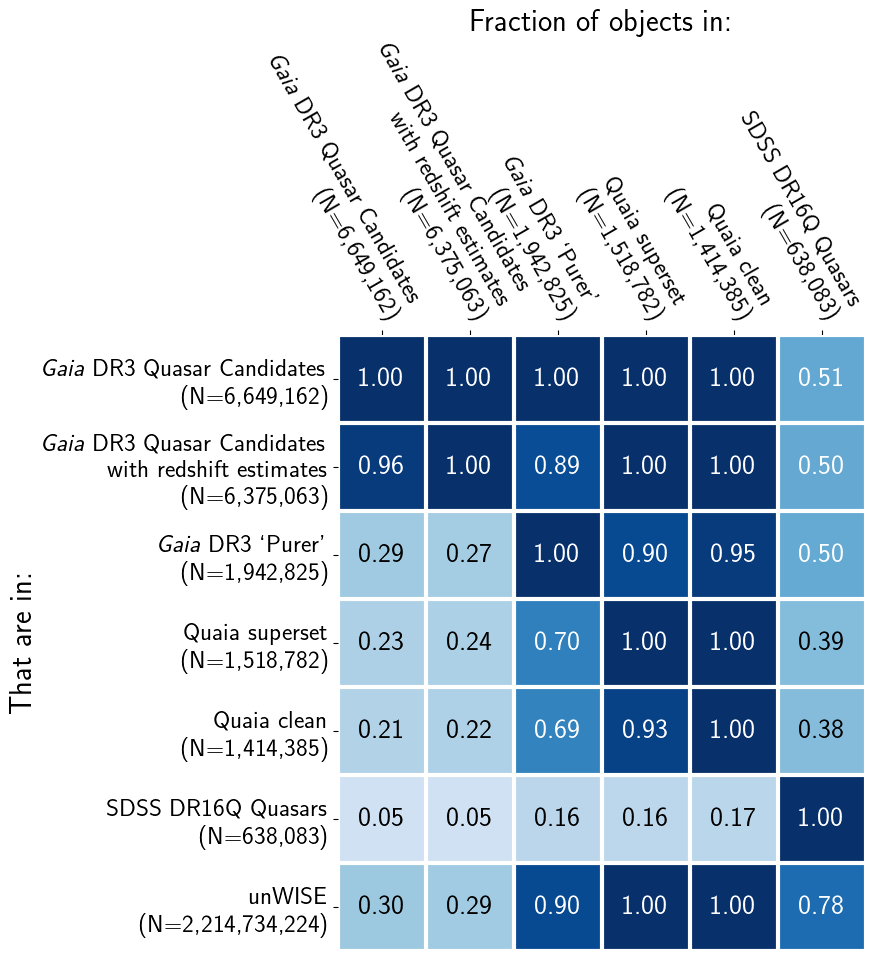
\includegraphics[width=0.6\textwidth]{frac_matrix.png}
    \caption{A summary of the overlaps between the various data sets and subsamples used in this work. The values describe the fraction of objects in each column's sample that are in each row's sample. Note that we only list \unWISE as a row because the inverse is not relevant to this work.}
    \label{fig:frac_matrix}
\end{figure}

\subsection{The \Gaia DR3 quasar candidate sample}
\label{sec:data_gaia}

\begin{figure}
    \centering
    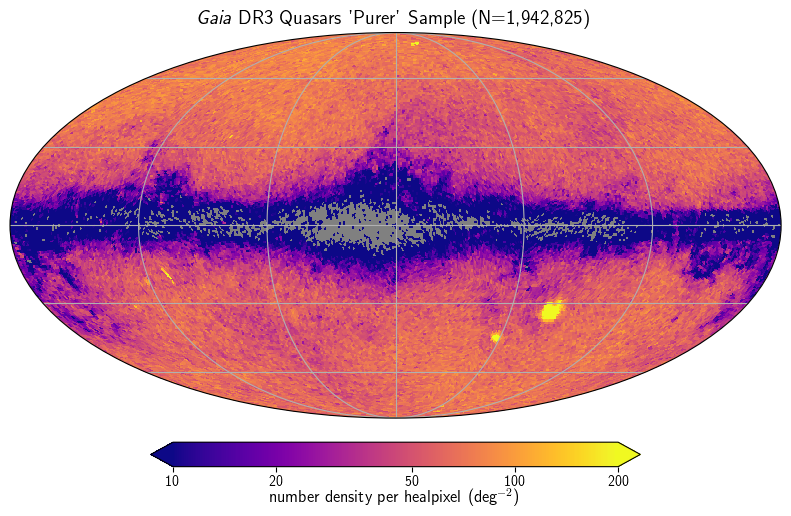
\includegraphics[width=0.6\textwidth]{gpurer_2d.png}
    \caption{Sky distribution of the quasar candidates in the \Gaia DR3 ``purer'' quasar sample, in Galactic coordinates and displayed using a Mollweide projection.}
    \label{fig:gaia_2d_purer}
\end{figure}

While performing its all-sky survey of the Milky Way, the \Gaia satellite \citep{gaia_collaboration_gaia_2016} also observed millions of extragalactic objects.
These sources---both quasar and galaxy candidates---were first released in \Gaia DR3 \citep{gaia_collaboration_gaia_2022, gaia_collab_gaia_2022}.
\Gaia obtained BP/RP spectra of the sources, which are low-resolution spectra with relatively narrow wavelength ranges; the blue photometer (BP) covers 330-680 nm and has $30 \leq R \leq 100$ and the red photometer (RP) covers 640-1050 nm \citep{carrasco_internal_2021} with $70 \leq R \leq 100$.
The raw spectra are not released by \Gaia (besides a small subsample---the rest will be released in \Gaia DR4), but redshift estimates and other derived information are contained in the catalogs.

The quasar candidates were selected based on multiple classifiers and criteria, described in detail in \cite{gaia_collab_gaia_2022}.
The majority (5.5 million) of the quasar candidates were identified with the Discrete Source Classifier (DSC) module (detailed in \cite{delchambre_gaia_2022}, a machine learning model that takes as input the source's BP/RP spectrum, $G$-band magnitude, $G$-band variability, parallax, and proper motion, and outputs a class label based on \SDSS spectroscopic classifications.
Given these \SDSS labels, the results of this module will inherit many of the same selection effects as \SDSS, such as missing highly reddened quasars.
DSC is estimated to have a completeness of over $90\%$ and a purity of around $24\%$ for quasars.
Another machine learning model selected over 1 million sources were contributed based on their variability, as active nuclei have time-variable accretion; the model inputs were statistics of time series data in all \Gaia bands as well as photometric and astrometric quantities, as detailed in \cite{rimoldini_gaia_2023}. 
Additionally, a set of nearly 1 million sources were selected based on their surface brightness profile; this selection used existing major quasar catalogs to compile an initial list of sources, which were then processed by the \Gaia surface brightness profile module \cite{ducourant_gaia_2022}.
This module included quasars in the candidates catalog which passed certain criteria, including having \Gaia observations covering $>86\%$ of the source's surface area and a confident assessment (positive or negative) of host galaxy presence.
Finally, the 1.6 million sources used to define the \Gaia-CRF3 celestial reference frame were contributed, which are based on cross-matches of \Gaia to external quasar catalogs.
A large fraction of sources are identified as quasars by multiple of these methods; the overlapping contributions are shown in Figure 3 of \cite{gaia_collab_gaia_2022}.
The full quasar candidate sample contains \val{N_gall} sources\footnote{The \Gaia DR3 quasar candidates sample, and all other \Gaia data, can be downloaded at \url{https://gea.esac.esa.int/archive}.}, selected for high completeness, but with a low purity estimated to be around 52\% \citep{gaia_collab_gaia_2022}.
We show the overlaps between this \Gaia quasar candidate sample and other samples and subsamples used and constructed in this work in Figure~\ref{fig:frac_matrix}.

Most of the quasar candidates (\val{N_gall_wqsoc}) are assigned redshifts using the Quasar Classifier (QSOC) module, which uses a chi-squared approach on the quasars' BP/RP spectra compared to composite spectra from \SDSS DR12Q \citep{delchambre_gaia_2022}.
We refer to these \Gaia redshift estimates as $\zgaia$.
Many of these redshifts are determined by a single line due to the narrow spectral range, resulting in aliasing issues when lines are misidentified (see Figure 15 in \cite{delchambre_gaia_2022}).
% these numbers are cited in delchambre paper, so not filled in automatically
An estimated 63.7\% of the redshifts have $|\Dz| < 0.1$, increasing to 97.6\% for quasar candidates with no redshift warning flags (this is the case for nearly $80\%$ of quasars with $G<18.5$, but decreases to less than 20\% for $G>19.5$).

\cite{gaia_collab_gaia_2022} provides a query to select a purer subsample of the quasar candidates.
It requires higher quasar probability thresholds from the various classifiers and excludes surface-brightness-selected galaxies that have close neighbors.
This results in \val{N_gpurer} sources with an estimated purity of 95\%; 1.7 million of these have Gaia redshifts. 
The sky distribution of this sample is shown in Figure~\ref{fig:gaia_2d_purer}.
The sample has a low density in the galactic plane, because the selection was trained on the \SDSS quasar sample which does not contain reddened sources (as it is based on a color selection), and overdensities around the Magellanic Clouds, as the sample still contains stellar contaminants.

For our analysis, we start with the full quasar candidate sample, rather than the ``purer'' sample or cutting on other \Gaia pipeline flags, to allow for higher completeness and minimize reproducing biases; we compare our catalog to the \cite{gaia_collab_gaia_2022} purer subsample in \S\ref{sec:comparison}.
We construct a \emph{superset} that contains all of the information needed for catalog construction: we require that sources are in the \Gaia quasar candidates table, have \Gaia $G$, $BP$, and $RP$ measurements, have \unWISE $W1$ and $W2$ observations (described in \S\ref{sec:data_wise}), have \Gaia-estimated QSOC redshifts, and make a maximum $G$-magnitude cut of $G < \Gmax$.
This magnitude cut was chosen to be slightly deeper than our desired catalog magnitude limit of $G<\Ghi$, in order to provide a buffer for redshift estimation.
This results in a superset with \val{N_gsup} sources.
We call our final catalog the \catalog (\cat), so we refer to this as the \cat superset.


\subsection{The \unWISE Quasar Sample}
\label{sec:data_wise}

We use the \unWISE survey to contribute infrared (IR) photometry to \Gaia sources \citep{lang_unwise_2014,meisner_unwise_2019}.
The \unWISE coadds combine data from NEOWISE \citep{mainzer_preliminary_2011} with the original WISE \citep{wright_wide-field_2010} survey, providing a time baseline fifteen times longer.
Compared to the original \textsl{AllWISE} catalog, \unWISE has deeper imaging and improved modeling of crowded fields.
The \unWISE catalog \citep{schlafly_unwise_2019} contains measurements in the $W1$ (3.4 $\mu$m) and  $W2$ (4.6 $\mu$m) bands for over 2 billion sources.
We do not use the $W3$ and $W4$ bands as these do not go as deep as we need.
We perform a cross-match of the \Gaia quasar candidate sample to \unWISE sources within 1''\footnote{We use NOIRLab's cross-match service to perform this operation, available at \url{https://datalab.noirlab.edu/xmatch.php}.}.
We also cross-match the \SDSS training and validation samples (\S\ref{sec:data_sdss_quasars}, \S\ref{sec:data_contaminants}) to \unWISE.

When combined with optical photometry, \unWISE IR color information is very useful for identifying quasars and distinguishing them from contaminants.
This photometry also contains useful redshift information; recent approaches to estimate redshifts from photometry with neural networks achieve a mean $|\Dz|\sim 0.22$ \citep{yang_quasar_2017, jin_efficient_2019, kunsagi-mate_photometric_2022}.
In our case of redshift estimates from narrow-range BP/RP spectra, we expect IR photometry to add information that can break line identification degeneracies in order to improve estimates.
We incorporate the $W1$ and $W2$ bands into both our quasar selection (\S\ref{sec:decontam}) and redshift estimation (\S\ref{sec:redshifts}) procedures.


\subsection{The \SDSS DR16 quasar sample}
\label{sec:data_sdss_quasars}

The Sloan Digital Sky Survey released the largest spectroscopic quasar catalog in DR16\footnote{The \SDSS DR16Q quasar catalog is publicly available at \url{https://www.sdss.org/dr16/algorithms/qso_catalog}.} \citep{lyke_sloan_2020}.
It combines new sources from the extended Baryon Oscillation Spectroscopic Survey (eBOSS), part of \textsl{SDSS-IV}, with previously observed sources from the earlier \SDSS campaigns.
The catalog contains 750,414 quasars, with an estimated 99.8\% completeness and $98.7-99.7$\% purity.
We remove sources with redshift warnings, \texttt{ZWARNING}!=0, as well as a handful of sources with unreasonably low or negative redshift estimates ($z<0.01$). 
This results in \val{N_sqall} sources, which is the sample shown in Figure~\ref{fig:frac_matrix}.
We cross-match these with the \Gaia catalog, as well as \unWISE (\S\ref{sec:data_wise}), using a maximum separation of 1'' on the sky.
We remove sources with fewer than 5 observations in $BP$ (\texttt{phot\_bp\_n\_obs}) or $RP$ (\texttt{phot\_rp\_n\_obs}), following \citep{bailer-jones_dsc_2021}, as well as sources that are duplicated in the \SDSS star or galaxy samples (\S\ref{sec:data_contaminants}) 
This results in \val{N_squasars_unwise} sources with both \Gaia and \unWISE observations that pass these criteria.

We use these to calibrate the cuts to make to decontaminate our sample (\S\ref{sec:decontam}); for this purpose we only keep sources that are also in the \cat superset (sources that are in the \Gaia quasar candidates table, have all necessary \Gaia and \unWISE photometry, \Gaia-estimated QSOC redshifts, and $G < \Gmax$).
This sample contains \val{N_squasars_sup} quasars.
We also use this sample (after applying the cuts described in \S\ref{sec:decontam}) to train our redshift estimation model (\S\ref{sec:redshifts}).
While this spectroscopic sample has quite high completeness and accurate redshift information, we note that it is still imperfect, contains selection effects, and represents only a particular definition of a quasar; these issues will propagate to our catalog.


\subsection{Contaminant samples: galaxies and stars}
\label{sec:data_contaminants}

To guide the decontamination of our catalog (\S\ref{sec:decontam}), we compile known contaminant samples, namely galaxies and stars.
For the galaxy sample, we use \SDSS spectroscopic galaxies from DR18\footnote{\SDSS DR18 data can be accessed at \url{https://skyserver.sdss.org/CasJobs/jobdetails}.}.
Following \citep{bailer-jones_dsc_2021}, we include all galaxies with class label \texttt{GALAXY} in the \texttt{SpecObj} table, exclude galaxies with subclass labels \texttt{AGN} or \texttt{AGN BROADLINE}, and exclude sources with redshift warnings, \texttt{zWarning=0}.
We cross-match these with \Gaia DR3 and \unWISE with a 1'' radius, and remove sources with fewer than 5 observations in $BP$ or $RP$, as for the \SDSS quasars.
We also remove apparent stellar contaminants from the galaxies sample with the cut in $G-RP$ and $BP-G$ from equation (1) of \cite{bailer-jones_quasar_2019}, and additionally remove sources duplicated in the \SDSS quasar or star samples.
This leaves \val{N_sgals_unwise} cross-matched \SDSS galaxies in our sample; \val{N_sgals_sup} of these are in the \cat superset.

For the star sample, we also use \SDSS DR18 sources, selecting objects with class label \texttt{STAR} in the \texttt{SpecObj} table.
As for the quasars and galaxies, we cross-match these with \Gaia DR3 with a 1'' radius and remove sources with fewer than 5 observations in BP or RP, and remove sources duplicated in the other samples.
This results in a stellar sample with \val{N_stars_unwise} cross-matched \SDSS-\Gaia stars, with \val{N_sstars_sup} of these in the superset.

For the decontamination procedure, we also compile a sample of sources in or near the LMC or SMC, as most of these will be stellar contaminants but have different properties than the \SDSS star sample.
To do this, we select all sources in the \Gaia quasar candidates table that are within 3 degrees of the center of the LMC or 1.5 degrees from the center of the SMC.
While this may include non-MC stars, we have chosen these fairly narrow radii in order to capture mostly MC stars and few potential quasars.
Additionally requiring that these have \unWISE photometry, this gives \val{N_mcs_unwise} MC-adjacent stars; \val{N_mcs_sup} are in the superset.


\section{Catalog construction}
\label{sec:construction}

\subsection{Decontamination with proper motions and \unWISE colors}
\label{sec:decontam}

\begin{figure}
    \centering
    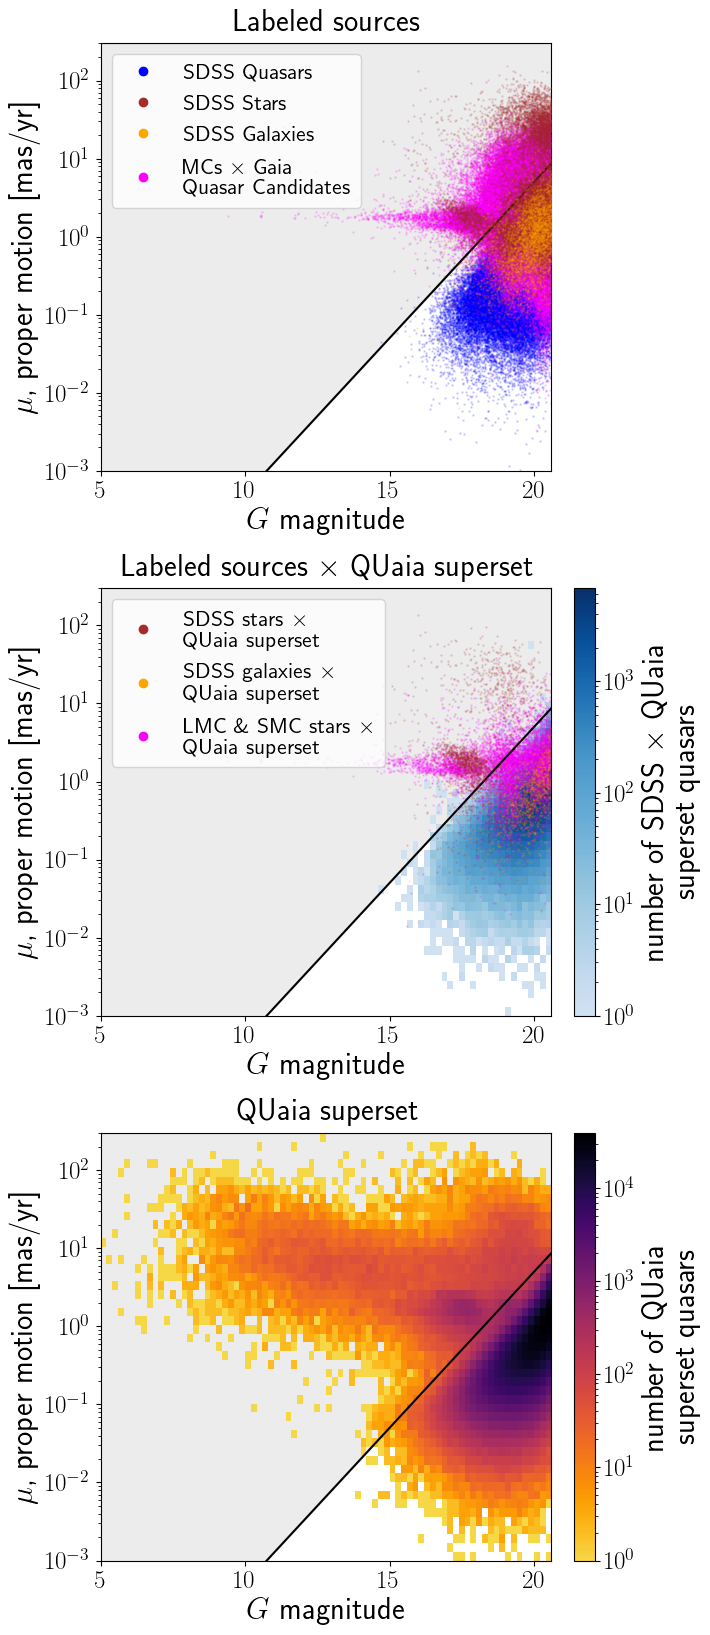
\includegraphics[width=0.42\columnwidth]{G_pm.png}

    \caption{Proper motion $\mu$ vs. $G$ magnitude  for two different sets of sources. The black line shows the cut we make; the shaded gray region is excluded from the catalog. \emph{Top:} The sources for which we have labels (\SDSS data as well as sources near the LMC and SMC in the \emph{Gaia} quasar candidates sample) that are also in the \cat superset (\Gaia DR3 quasar candidates that have all necessary photometry, \Gaia redshift estimates, and $G<\Gmax$). \emph{Middle:} Sources in the top row that are also in the \cat superset (\Gaia DR3 quasar candidates that have all necessary photometry, \Gaia redshift estimates, and $G<\Gmax$). \emph{Bottom:} The superset of quasar candidates from which the \catalog is constructed. The proper motion cut includes nearly all \SDSS quasars in the superset while excluding a large number of stars.} 
    \label{fig:G_pm}
\end{figure}

The full \Gaia quasar candidate sample is known to contain a significant fraction of contaminants (stars and other non-quasars, such as galaxies).
We make an initial cut on proper motion $\mu$, as quasars should have negligible proper motions due to their large distances.
The value of $\mu$ has a dependence on $G$, so we make a cut in this space.
To guide this cut, we use labeled sources: \SDSS quasars, \SDSS galaxies, \SDSS stars, and \Gaia LMC- and SMC-adjacent stars, as described in \S\ref{sec:data_sdss_quasars} and \S\ref{sec:data_contaminants}.
The $G$-$\mu$ distributions of these sources are shown in the top panel of Figure~\ref{fig:G_pm}.
In the middle panel, we show the intersection of these labeled sources with our \cat superset, which consists of sources in the \Gaia quasar candidates table that have \Gaia redshift estimates, complete \Gaia and \unWISE photometry, and are below $G<\Gmax$.
We see that the \SDSS quasars tend to have much smaller proper motions than the other types of sources, with a very linear edge to the $G$-dependence at the high proper motion side of the distribution.
Based on this, we choose the cut
\begin{equation}
    \mu < 10^{0.4\,(G-18.25)} ~.
\end{equation}
At $G=18.25$, this corresponds to $\mu < \sim2.5$, and allows for less harsh cuts at deeper magnitudes given the typically less precise astrometry.
We show this cut overlaid over the \catalog superset in the lower panel of Figure~\ref{fig:G_pm}; based on the labeled data, we can clearly pick out the populations.
The proper motion cut excludes \val{N_removed_pmcut}, $\val{p_removed_pmcut}\%$ of the superset.

\begin{figure*}[p]
    \centering
    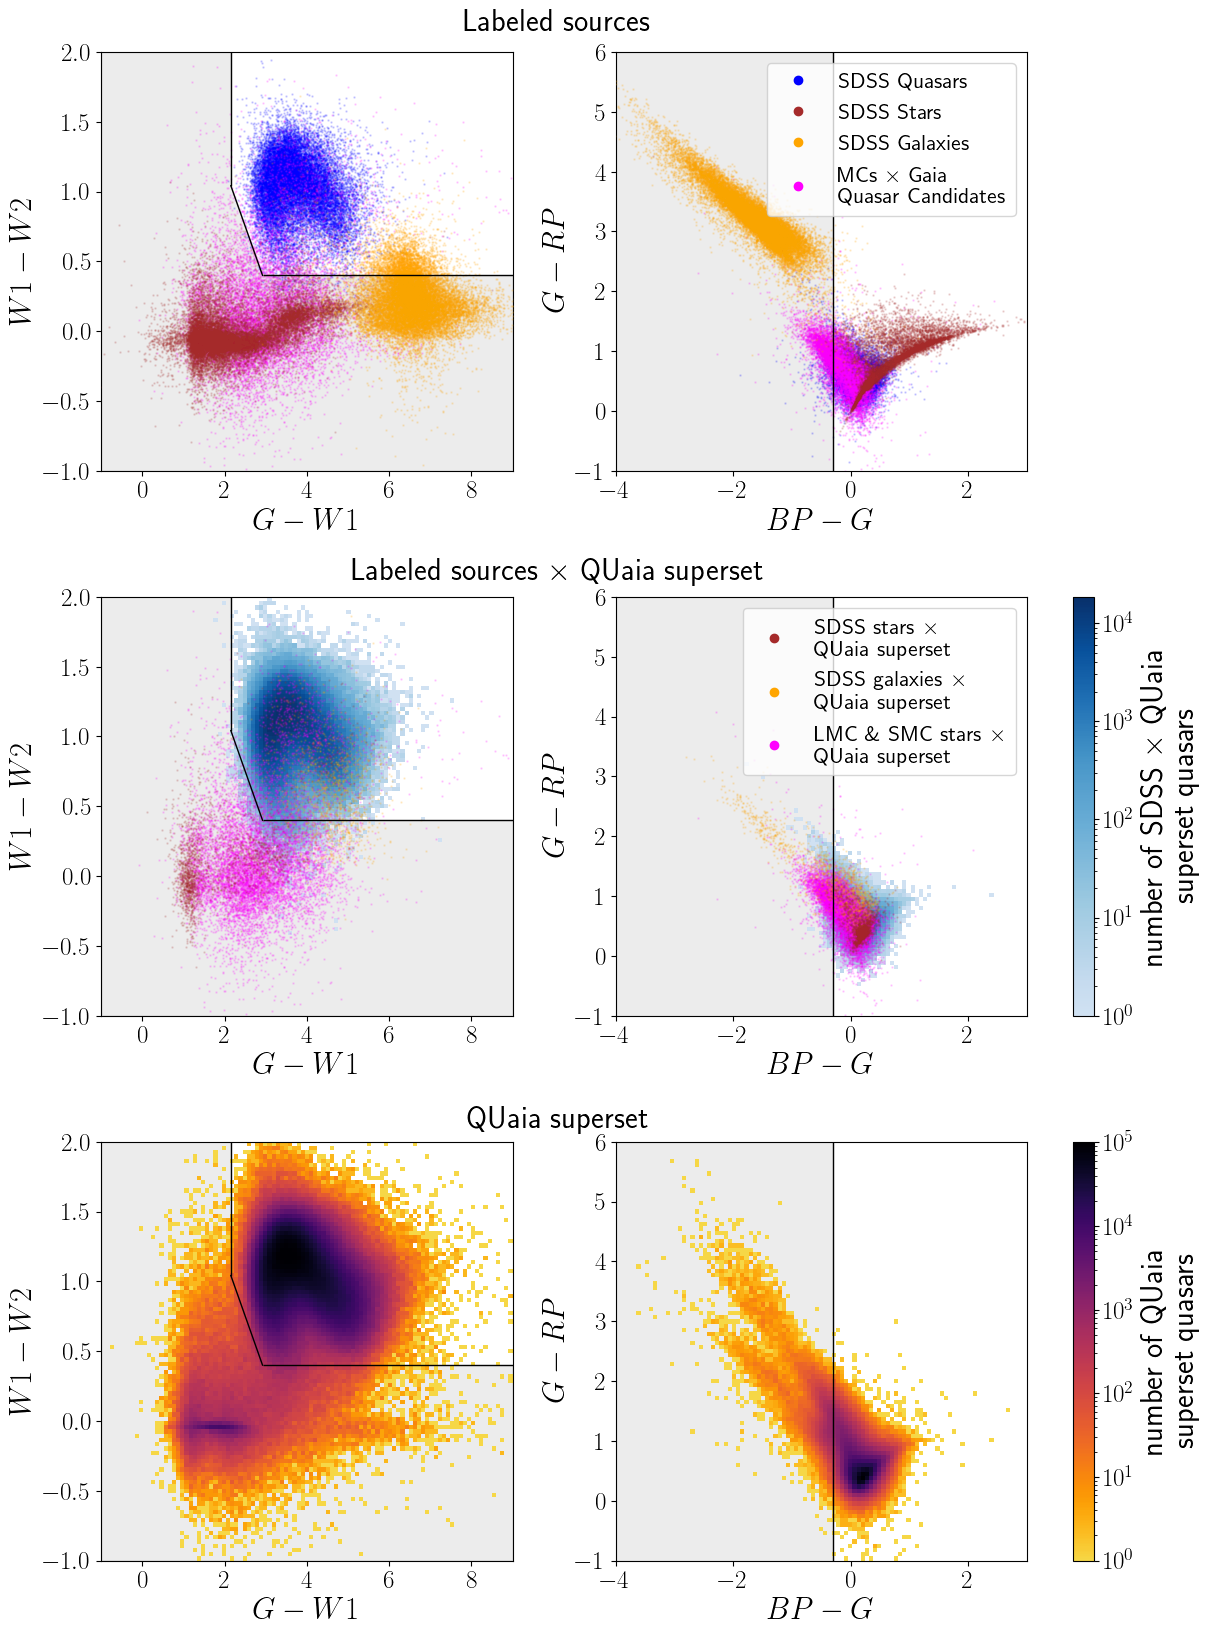
\includegraphics[width=0.8\textwidth]{color_color.png}

    \caption{Color-color plots of three different sets of sources. The left column shows $W1-W2$ vs. $G-W1$ color, and the right column shows $G-RP$ vs. $BP-G$ color. The black lines show the cuts we make; the shaded gray region is excluded from the catalog. The rows have the same samples as in Figure~\ref{fig:G_pm}, except that in the top row only 20,000 of each type of \SDSS source is shown for clarity. In both color-color projections, the labeled sources are mostly localized in particular regions of parameter space, and we can see these populations somewhat clearly in the \cat superset.} 
    \label{fig:color_color}
\end{figure*}

We next determine color cuts based on \Gaia and \unWISE photometry.
Generally, stars and galaxies are dim in redder, IR wavelengths compared to AGN.
For instance, the eBOSS target selection involved a cut in the optical-IR, involving the \SDSS $g$-, $r$-, and $i$-bands and WISE $W1$ and $W2$ bands (as $W3$ and $W4$ have a significant difference in depth) \citep{myers_target_2022}. 

In Figure~\ref{fig:color_color}, we show color-color distributions for the same samples as in Figure~\ref{fig:G_pm}.
The left panel shows $W1-W2$ vs. $G-W1$ color, and the right column shows $G-RP$ vs. $BP-G$ color.
The top row, with the full labeled samples, shows that different types of sources tend to be localized to different areas of this parameter space (we show only a subset of each type for clarity).
In particular, the colors involving \unWISE (left panel) separate out the source types relatively clearly, demonstrating the importance of the \unWISE cross-match: \SDSS quasars have high $W1-W2$ and $G-W1$ color, while galaxies have low $W1-W2$ and high $G-W1$, and stars (both \SDSS stars and stars near the LMC and SMC) are lower in both colors.
In \Gaia color-color space, galaxies tend to have lower $BP-G$ and higher $G-RP$ colors than the other types of sources.
In the middle row of Figure~\ref{fig:color_color}, showing the intersection of the labeled sources with the \cat superset, we see that the superset restrictions have eliminated many of the sources, especially \SDSS galaxies and stars, though a significant number remain.
(We note that it is possible that some of these \SDSS galaxies do host AGN though they weren't classified as such by \SDSS.)
The \cat superset is shown in the bottom panel; we can see clear populations of quasars, stars, and galaxies lining up with the labeled sources.
Importantly, we can see the effect of the stricter \SDSS color selection in the red (high $G-W1$) region of parameter space into which the \Gaia quasar candidates extend, but are not represented in the \SDSS sample in the above panels.

We choose to apply linear cuts in these colors to decontaminate the sample.
While other works (e.g. \citealt{hughes_quasar_2022}) train classifiers to determine which objects are true quasars, we opt for simpler cuts for ease of reproducibility and to avoid imposing the same selection effects as \SDSS, especially as the strict \SDSS color selection may exclude significant regions of quasar parameter space.
We choose four cuts based on the distribution of sources in color-color space. 
The first is in $W1-W2$, which has been shown to be useful for distinguishing quasars; for instance, \cite{nikutta_meaning_2014} demonstrated that a small cross-matched \SDSS quasar sample has high $W1-W2=1.2 \pm 0.16$, while other types of objects---namely star-forming and AGN galaxies, luminous red galaxies and stars---have lower $W1-W2$.
Stars tend to have the lowest $W1-W2$, with a mean of $W1-W2=-0.04 \pm 0.03$, so a cut in $W1-W2$ is a reliable way to filter out stellar contaminants.
We add a cut in $G-W1$ to filter out the bulk of the stars (including the LMC and SMC), and another in $BP-G$ to cut out the galaxy contaminants.
Finally, we find that these single-color cuts were not sufficient to remove all of the LMC and SMC, so we add an additional diagonal cut in $W1-W2$ and $G-W1$, choosing a reasonable slope.

We optimize the values (intercepts) of these four cuts with a grid search, trying values spaced out by 0.1 magnitudes.
We note that while we show the full samples in Figure~\ref{fig:color_color}, in practice we make the proper motion cut before optimizing the color cuts.
We choose that color cuts that maximize our objective function $\mathcal{L}$,
\begin{equation}
    \mathcal{L} = N_\text{q} - \lambda_\text{s} \, N_\text{s} - \lambda_\text{g} \, N_\text{g} - \lambda_\text{m} \, N_\text{m} ~,
\end{equation}
where $N_\text{q}$ is the number of true quasars that make it into the catalog, $N_\text{s}$ \SDSS stars, $N_\text{g}$ \SDSS galaxies, and $N_\text{m}$ LMC and SMC stars, and the $\lambda$ parameters balance the relative ratios of each.
We choose $\lambda_\text{s}=3$, $\lambda_\text{m}=5$, and $\lambda_\text{g}=1$.

The optimal cuts for the objects to keep in the catalog are
\begin{equation}
\begin{split}
    (G-W1) &> 2.15 \\ (W1-W2) &> 0.4 \\ (BP-G) &> -0.3 \\ (G-W1) + 1.2\,(W1-W2) &> 3.4
    %{\colorcutstr} ~.
\end{split}
\end{equation}
These are shown as the black lines in all panels of Figure~\ref{fig:color_color}, with the grey shading indicating exclusion regions.
These cuts, as well as the proper motion cuts described above, exclude ${\sim}\val{p_cut_gsup_gclean}\%$ of the superset, resulting in \val{N_gclean} quasars in our ''decontaminated'' sample.
We apply an additional magnitude cut of $G<\Ghi$ to reduce edge effects in our redshift estimation; this constitutes our deep sample, with \val{N_gcathi} sources.
We refer to this as the \catalog (\cat) in the rest of this work.
The catalog becomes less clean and reliable as we push to deeper magnitudes---due to less precise measurements and stronger systematics, notably the \Gaia scanning pattern---so we produce a version of the catalog with $G<\Glo$ to ensure a cleaner sample.
This brighter catalog has \val{N_gcatlo} sources, and we report most of our results on this sample throughout the rest of this work.


\subsection{Spectro-photometric redshifts with \unWISE and \SDSS}
\label{sec:redshifts}

\begin{figure*}
    \centering
    \subfloat[\label{fig:zgaia_zsdss}]{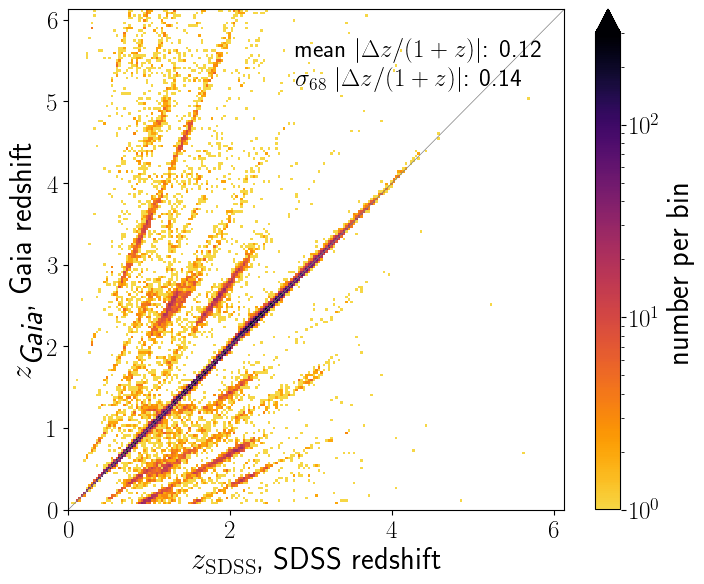
\includegraphics[width=0.45\textwidth]{redshift_zgaia_vs_zdss_Ghi.png}}
    \hspace{5ex}
    \subfloat[\label{fig:zspz_zsdss}] {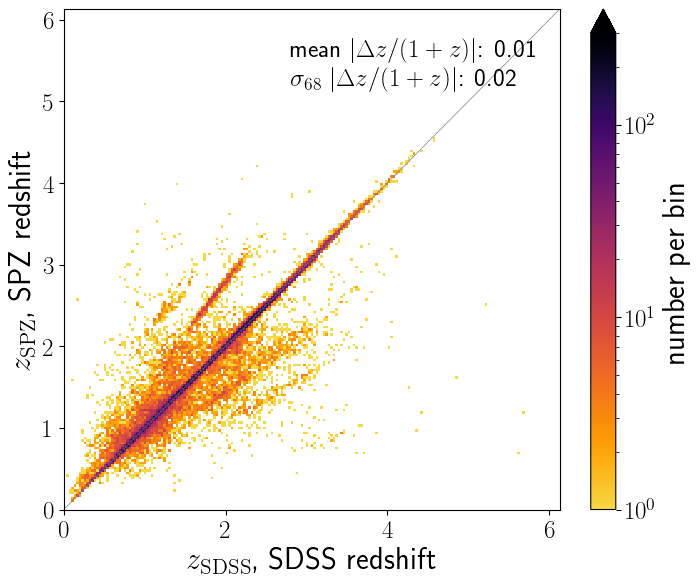
\includegraphics[width=0.45\textwidth]{redshift_zspz_vs_zdss_Ghi.png}}
    \caption{(a) \Gaia redshift estimate $\zgaia$ vs. \SDSS (''true'') redshift $\zsdss$ for a test set of sources in our quasar catalog \cat with $G<\protect\Ghi$. (b) Our estimated spectro-photometric (SPZ) redshifts $\zspz$ vs. $\zsdss$ for the same sample. The $\zspz$ redshifts, which are based on a \knn model, significantly decrease both the bias and scatter, as well as catastrophic outliers and unreasonably high redshift estimates. The one-to-one line (perfect accuracy) is shown in grey; note that the color bar is on a log scale, and that a majority of the sources in both cases lie along this line.}
    \label{fig:zsdss_comp}
\end{figure*}

We use \unWISE and \SDSS data to improve the redshift estimation of the sources.
Figure~\ref{fig:zgaia_zsdss} shows the redshifts estimated by the \Gaia QSOC pipeline $\zgaia$ compared to the \SDSS redshifts $\zsdss$ for a test sample of sources from \cat with $G<\Ghi$; note that the 2D histogram is plotted in log-space to show the outliers more clearly.
We find that of the \Gaia redshifts $\zgaia$, $\val{p_acc_zgaia_dzhi_Glo}\%$ ($\val{p_acc_zgaia_dzmid_Glo}\%$) agree to $|\dz|<\val{dzhi}$ ($\val{dzmid}$).
A significant fraction of $\zgaia$ are highly precise: $\val{p_acc_zgaia_dzlo_Glo}\%$ agree with \SDSS to $|\dz|<\val{dzlo}$.
We also clearly see bands of incorrect estimation due to line aliasing issues.
Additionally, in the cross-matched sample, nearly all of the very high $\zgaia$ estimates ($z>4.5$) are shown to be incorrect in comparison to \SDSS.

We train a $k$-Nearest Neighbors (\knn) model to estimate improved redshifts.
(We also tried other models including XGBoost and a multi-layer perceptron, and found that the \knn outperformed both overall.)
We include all sources in our decontaminated catalog (\S\ref{sec:decontam}) which goes out to $G<\Gmax$, in order to have a buffer beyond our desired $G<\Ghi$ sample to reduce edge effects from the training set.
The features that we train on are: the \Gaia redshift $\zgaia$, colors constructed using \Gaia and WISE photometry ($G-RP$, $BP-G$, $BP-RP$, $G-W1$, $W1-W2$), the \Gaia $G$-band magnitude, and the dust reddening $E(B-V)$ at the location of the source.
(We find that including the rest of the photometry does not make a difference in the results.)
The reddening is determined with the \citep{schlafly_measuring_2011} dust map\footnote{The dust map was accessed with the python package \url{https://dustmaps.readthedocs.io}}.
The labels are the \SDSS redshifts, $\zsdss$.

We use as our labeled data sources from the cross-matched \SDSS DR16Q sample (\S\ref{sec:data_sdss_quasars}) that are also in our decontaminated catalog \cat, so that we train on sources drawn from the same distribution to which we will apply the model; this is \val{N_sqclean} sources.
We apply a 70\%/15\%/15\% train/validation/test split.
We build a $k$-d tree on the training set features using the \texttt{KDTree} implementation of \texttt{sklearn}.
At the prediction stage, we access the $K$ nearest neighbors of each input feature vector, first excluding neighbors with zero distance in feature-space (i.e. neighbors that are in the training set).
We assign the predicted label to be the median $\zsdss$ of the $K$ nearest neighbors, and the uncertainty to be the symmetrized inner 68\% error of those neighbors.
We use the validation set to tune $K$, and choose the value that maximizes the fraction of predicted redshifts with $|\dz|<\val{dzmid}$, which is $K=27$; we note that this value only varies at the $\sim$1\% level for values $15 < K < 50$, and is similar for other choices of $|\dz|$. 
Finally, we apply the model to the full \cat and output \knn redshift estimates, $\zknn$, for each source.

\begin{figure}
    \centering
    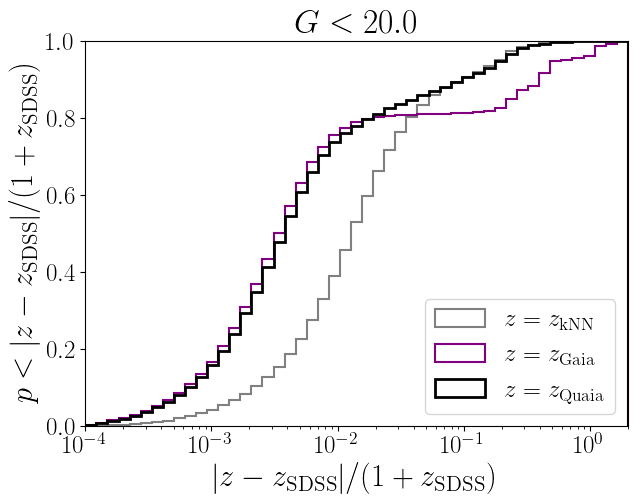
\includegraphics[width=0.55\columnwidth]{redshift_error_cumulative_Glo.png}
    \caption{The cumulative distribution of redshift errors for \cat test set sources with $G<\protect\Glo$, considering \SDSS spectroscopic redshifts $\zsdss$ as ground truth, for estimates directly from our \knn model (grey), the original $\zgaia$ redshifts (purple), and our final $\zspz$ estimates (black) based on a combination of the other two. Our SPZ redshifts have far fewer outliers and similar precision compared to the \Gaia estimates.}
    \label{fig:z_error_cumulative}
\end{figure}

The results are shown in Figure~\ref{fig:z_error_cumulative}, which shows the cumulative distribution of errors $|\dz|$ for $\zknn$ compared to that of $\zgaia$ (with $\zsdss$ as the truth) for the test set with $G<\Glo$.
(The shapes are similar for $G<\Ghi$, just shifted to somewhat lower accuracy.)
We find that the $\zknn$ estimates have far fewer outliers than $\zgaia$.
However, the $\zgaia$ estimates tend to be more precise, as they use the full spectral information, while the \knn is essentially smoothing over the likeliest neighboring sources in feature space. 
We thus choose to combine the properties of both of these redshift estimates to obtain our final \emph{spectro-photometric} (SPZ) redshifts $\zspz$ in the following way.
For sources for which $\zspz$ and $\zgaia$ agree to $|\dz|<0.05$, we assign $\zspz = \zgaia$ to preserve the precision of the \Gaia estimate.
For sources for which $\zspz$ and $\zgaia$ differ by $|\dz|>0.1$, we assign $\zspz = \zknn$ to preserve accuracy.
In between these thresholds, we apply a smooth, linear transition to avoid hard features in our estimates.
These $\zspz$ estimates are also shown in Figure~\ref{fig:z_error_cumulative} compared to the ''true'' \SDSS redshifts, and we can see that these achieve nearly as high precision as $\zgaia$ while maintaining the high accuracy of $\zknn$.

Our $\zspz$ results for the test set are shown in Figure~\ref{fig:zspz_zsdss} compared to $\zsdss$, here shown for the full catalog depth $G<\Ghi$. 
We find that $\val{p_acc_zspz_dzhi_Ghi}\%$ ($\val{p_acc_zspz_dzmid_Ghi}\%$) of our SPZ redshifts agree to $|\dz|<\val{dzhi}$ $(\val{dzmid})$, and $\val{p_acc_zgaia_dzlo_Ghi}\%$ highly agree to $|\dz|<\val{dzlo}$.
We also give the mean and uncertainty of $|\dz|$ in the figure; our SPZ redshifts significantly decrease the bias and scatter.
The SPZ estimation corrected all of the very high-$z$ \Gaia estimates, and some of the intermediate-outlying aliasing effects.
We still have some catastrophic outliers due to line aliasing, but with our SPZ redshifts we find a reduction in the number of $|\dz|>\val{dzhi}$ (\val{dzmid}) outliers by \val{factor_reduction_outliers_dzhi_Ghi} (\val{factor_reduction_outliers_dzmid_Ghi}) compared to the \Gaia redshift estimates.


\begin{figure}
    \centering
    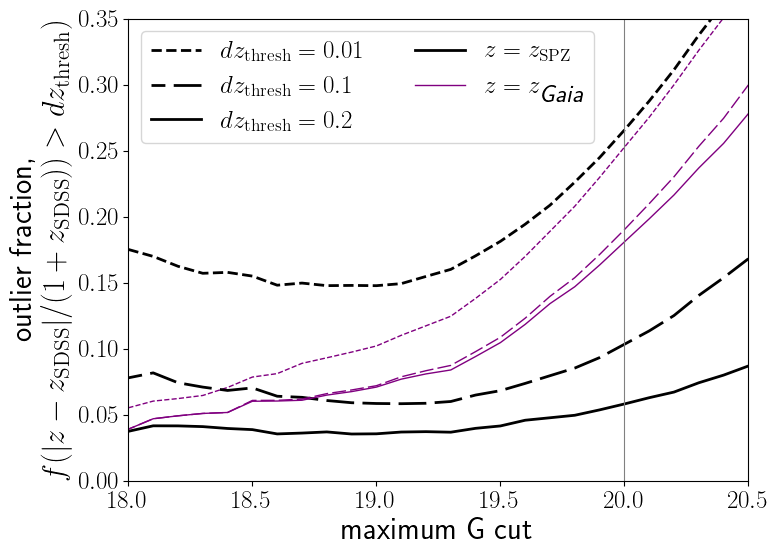
\includegraphics[width=0.55\columnwidth]{redshift_outliers_vs_Gmax.png}
    \caption{The fraction of outlying redshifts with $|\dz| > (\protect\val{dzlo}, \protect\val{dzmid}, \protect\val{dzhi})$, as a function of $G$ magnitude, for our redshift estimation test set. The SPZ redshifts are shown in black, and the \Gaia redshifts in purple. The fraction of outliers increases steeply with increasing $G$ for $G>19.5$ for both $\zspz$ and $\zgaia$, though the fraction of catastrophic outliers for $\zspz$ is significantly lower (and the dependence less steep) compared to $\zgaia$.}
    \label{fig:z_G_dep}
\end{figure}

We investigate the dependence of the redshift error on $G$-band magnitude in Figure~\ref{fig:z_G_dep}.
The fraction of redshifts with an error above a various thresholds is shown as a function of samples with given cut on $G$.
The errors are lowest at a bright magnitude cut of $G < \sim$$\val{Gbright}$; in this sample, sources with SPZ redshift estimates inaccurate to $|\dz|>\val{dzhi}$ (\val{dzmid}) comprise only $\val{p_outliers_zspz_dzhi_Gbright}\%$ ($\val{p_outliers_zspz_dzmid_Gbright}\%$) of the sample, and to the more stringent requirement of $|\dz|>\val{dzlo}$, $\val{p_outliers_zspz_dzlo_Gbright}\%$.
This outlier fraction increases steadily as fainter sources are included.
For $G<\Glo$, $\val{p_outliers_zspz_dzhi_Glo}\%$ ($\val{p_outliers_zspz_dzmid_Glo}\%$) are inaccurate to $|\dz|>\val{dzhi}$ $(\val{dzmid})$, and $\val{p_outliers_zspz_dzlo_Glo}\%$ for $|\dz|>\val{dzlo}$.
Compared to the \Gaia redshift estimates, the SPZ estimates $\zspz$ reduce the number of $|\dz|>\val{dzhi}$ (\val{dzmid}) outliers by \val{factor_reduction_outliers_dzhi_Glo} (\val{factor_reduction_outliers_dzmid_Glo}).
The choice of $G$ cut to use in a given analysis will depend on the nature of the analysis and its sensitivity to outliers. 
We also find that the fraction of errors increases slightly towards very bright magnitude cuts.
As this only occurs for our $\zspz$ and not the $\zgaia$ estimates, we speculate that this is due to low number statistics in the bright regime that lead to a low number of nearby neighbors in the \knn and thus poorer estimates.


\subsection{Selection Function Modeling}
\label{sec:selfunc_methods}

\begin{figure*}
    \centering

    \subfloat[\label{fig:systematics_dust}]{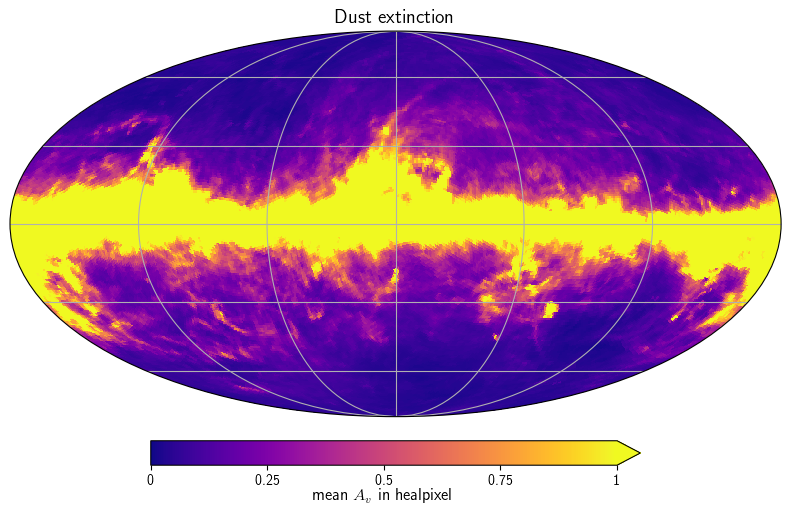
\includegraphics[width=0.45\textwidth]{systematics_map_dust.png}}
    \hspace{5ex}
    \subfloat[\label{fig:systematics_stars}]{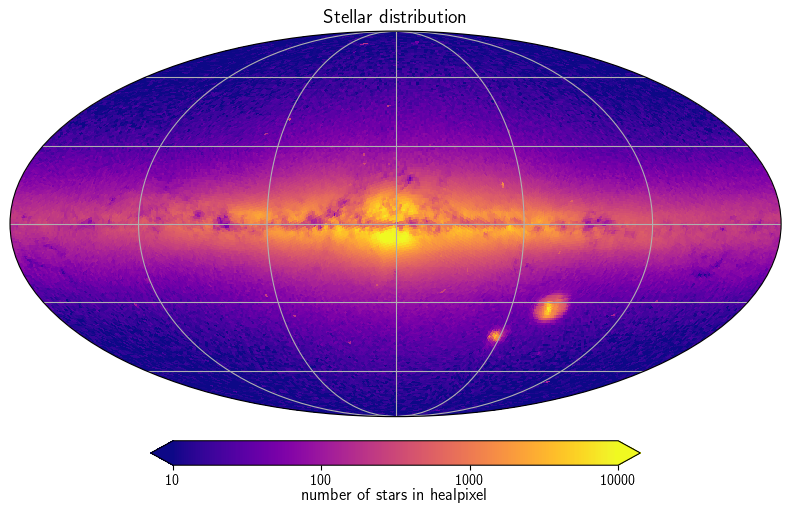
\includegraphics[width=0.45\textwidth]{systematics_map_stars.png}}
    
    \subfloat[\label{fig:systematics_mcs}]{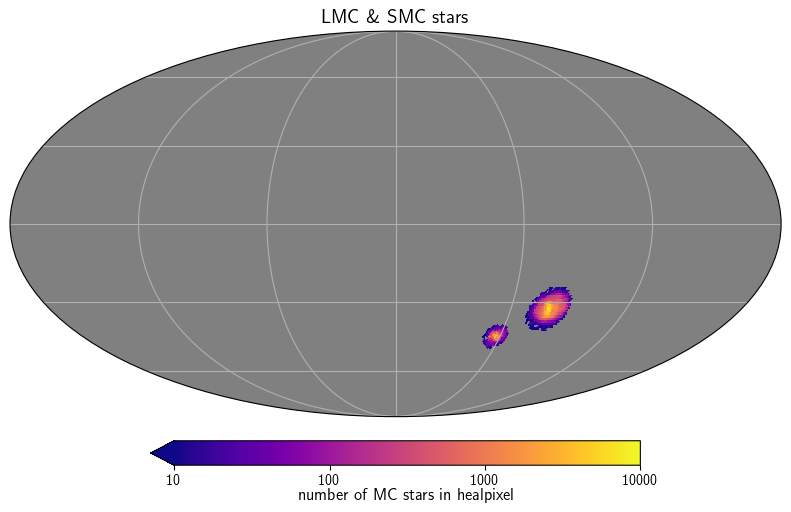
\includegraphics[width=0.45\textwidth]{systematics_map_mcs.png}}
    \hspace{5ex}    
    \subfloat[\label{fig:systematics_m10}]{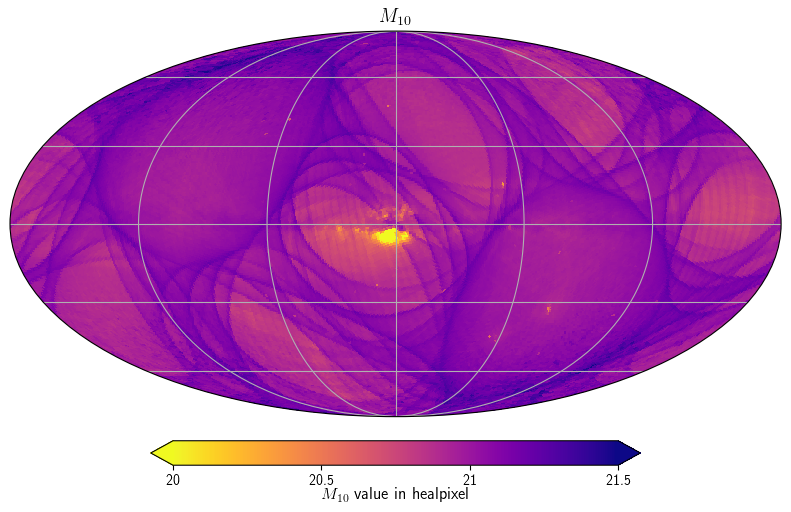
\includegraphics[width=0.45\textwidth]{systematics_map_m10.png}}

    \caption{The systematics maps used in the selection function model: (a) dust extinction based on \cite{schlafly_measuring_2011}; (b) the stellar distribution based on $\sim$10.6 million randomly selected \Gaia sources with $18.5 < G < 20$; (c) stars from the above panel belonging to the LMC and SMC, with the background subtracted; and (d) the quantity $M_{10}$, the median magnitude of sources with $\leq 10$ \Gaia transits, which encodes the scanning law and source crowding. Note that the color bar on the $M_{10}$ map is reversed, as high $M_{10}$ indicates a cleaner region, the inverse of the other maps.}
    \label{fig:systematics}
\end{figure*}

Observational and astrophysical effects impact which sources we observe and their properties; this is known as the selection function. 
As \Gaia is a space-based mission, it avoids many of the observational issues of ground-based surveys, such as seeing and airmass.
However, there are still significant selection effects: for our model, we consider dust, stellar density, and the \Gaia scan pattern.

We fit a selection function model to a particular version of the catalog, namely a particular maximum $G$.
We make a healpix map of the catalog with NSIDE=64 and count the number of observed catalog sources in each healpix pixel.
In the case of no selection effects (and under the assumption of isotropy), we would expect each pixel to contain roughly the same number of sources.
Our goal is to model the dependence between the number of sources per pixel and the various systematics.

The systematics maps (templates) we use are shown in Figure~\ref{fig:systematics}. 
We use the dust map of \cite{schlafly_measuring_2011}, and convert it to a healpix map of NSIDE=64.
To do this, we evaluate the reddening $E(B-V)$ at the centers of pixels of a high-resolution NSIDE=2048 healpixelization of the sphere.
We convert these to extinction values by multiplying by $R_V=3.1$, and then take the mean of all of these values within each healpixel target NSIDE=64 map.
This produces a smoothed dust extinction map on the desired scale.
The result is shown in Figure~\ref{fig:systematics_dust}; the extinction is highest around the galactic plane, with structure extending outwards.

For the stellar distribution, we randomly select $\sim$10.6 million \Gaia sources with $18.5<G<20$, the magnitude range of most of our quasar sample.
The vast majority of these will be true stars (though they will contain some other types of objects).
We count the number of stars per NSIDE=64 pixel; this is shown in Figure~\ref{fig:systematics_stars}.
We find that we require a separate map of the LMC and SMC to properly fit these regions, suggesting that the quasar catalog has a different dependence on the MCs than the galactic plane stellar distribution.
To do this we cut out a wide region around each MC (9 degrees in radius around the LMC and 5 around the SMC), and subtract the background, which we approximate using the horizontally mirrored region of the stellar distribution map.
This is shown in Figure~\ref{fig:systematics_mcs}.

For the \Gaia completeness, we use the quantity $M_{10}$ introduced by \cite{cantat-gaudin_empirical_2023}\footnote{This map can be accessed with the \texttt{gaiaunlimited} package, \url{https://gaiaunlimited.readthedocs.io}}.
$M_{10}$ is the median magnitude in a given sky patch of the \Gaia sources with $\leq 10$ transits across the \Gaia field of view; it incorporates the effects of both the scanning law and source crowding.
The actual completeness map derived by \cite{cantat-gaudin_empirical_2023} depends on both $M_{10}$ and $G$-band magnitude; however, this completeness is still extremely close to 1 for nearly all of the sky for $G=\Glo$, the limiting magnitude of our clean quasar catalog, due to the differences in the selection function and magnitude dependence for stars compared to quasars.
Thus we cannot use the completeness map directly, but we do still expect a dependence of the quasar selection function on the \Gaia scanning law, so use the $M_{10}$ map directly to capture this effect.
We down-sampled the map to NSIDE=64; this is shown in Figure~\ref{fig:systematics_m10}.


To model the selection function we use a Gaussian process, a flexible machine learning method for regression; for a detailed treatment, see \cite{RasmussenWilliams2006}.
(We first tried a linear model and found that it gave a very poor fit, as there are significant nonlinearities between the systematics and the catalog number density.)
We first scale the data: for the labels (number of \cat sources per pixel) we work in their logarithm, and only fit for the pixels with a nonzero number of sources.
For the stellar distribution and MC map templates, we also take the log of the number of quasars per pixel; for the MC map we first replace zeros with a very small value.
For all of the input feature maps, we take the mean-subtracted systematics values in order to use a zero-mean Gaussian process.
We assume a Poisson error on the labels (and apply the appropriate log transformation).
For the Gaussian process, we use the \texttt{george} software package \citep{Ambikasaran2016}. 
We use an exponential squared kernel $k$ of the form
\begin{equation}
    k(r^2) = \text{exp}\left(\frac{-r^2}{2}\right)~,
\end{equation}
where $r$ is the distance between points in feature space.
We train the Gaussian process on all of the data, optimizing the parameter vector using the BFGS solver.
We finally evaluate the predicted number of sources in each pixel.
Where there were no \cat sources in the label map, we fix the prediction to zero.

To convert this to a selection function in terms of the probability of inclusion of a source in the final catalog, we first identify ``clean'' pixels in the map having low dust extinction ($A_v < 0.03$), low star counts ($N_\mathrm{stars} < 15$), no MC stars, and high $M_{10}$ ($M_{10} > 21$); this results in 301 pixels.
We take the mean predicted number of quasars in these clean pixels, normalize the predicted source numbers by this mean, and then fix pixels with normalized values greater than 1 to exactly 1.
The result is a selection function map in terms of the probability of a source's inclusion in the catalog.
This fit must be done for each version of the catalog as it depends on the particular number density and distribution of sources, which depends most notably on magnitude.


\section{The Catalog: Results and Verification}
\label{sec:catalog}

\subsection{Properties of the catalog}
\label{sec:properties}

\begin{figure*}
    \centering
    \subfloat[\label{fig:gcatlo_2d}]{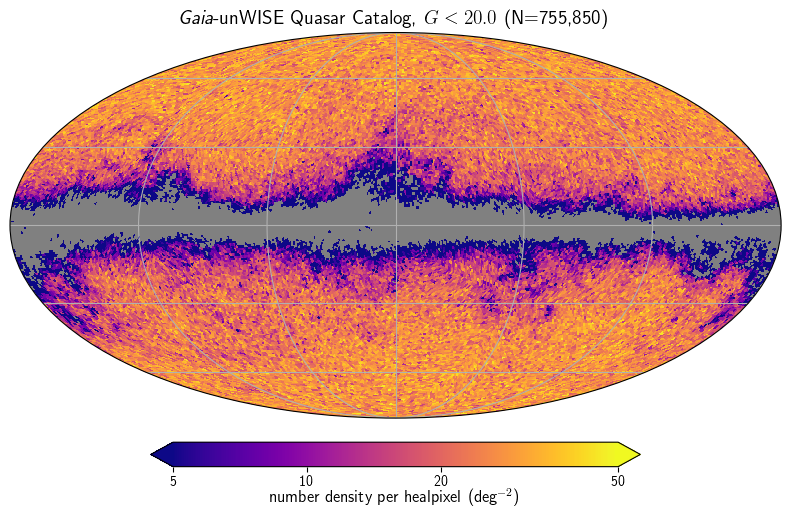
\includegraphics[width=0.8\textwidth]{gcatlo_2d.png}}
    
    \subfloat[\label{fig:gcathi_2d}]{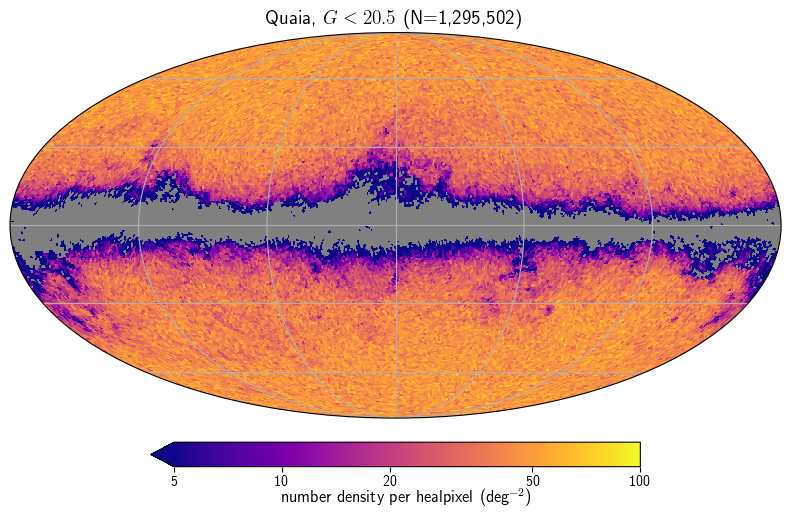
\includegraphics[width=0.8\textwidth]{gcathi_2d.png}}
    \caption{Sky distribution of our \catalog, in Galactic coordinates and displayed using a Mollweide projection. Panel (a) shows sources with $G<\protect\Glo$, the cleaner version with more reliable redshifts, and (b) shows the catalog down to its magnitude limit of $G<\protect\Ghi$.}
    \label{fig:gcat_2d}
\end{figure*}

Our \catalog consists of \val{N_gcatlo} (\val{N_gcathi}) quasar candidates with $G<\Glo$ $(\Ghi)$.
The sky distribution of \cat for each of these magnitude limits is shown in Figure~\ref{fig:gcat_2d}.
The catalog covers the full sky, besides the galactic plane, including the Southern sky---most of which is not well covered by other surveys (see the bottom panels of Figure~\ref{fig:2d_comp}, discussed further in \S\ref{sec:comparison}). 
The sky distribution is remarkably uniform, and the non-uniform imprints visually follow the selection effects that we incorporated into our selection function map, most notably the dust distribution (Figure~\ref{fig:systematics_dust}). 
\cat also does not show an obvious overdensity around the LMC and SMC (as the \Gaia purer sample does), as we have removed these with our decontamination procedure.
In fact, there is now a slight underdensity of sources near the LMC; this makes sense as some quasars in that sky region would be as they are blocked by the LMC, though it is possible we have somewhat over-corrected for this and removed some true quasars. 

The dearth of quasars in the galactic plane is due largely to dust extinction and stellar crowding, as well as the fact that the \SDSS training set quasars (for both the original \Gaia DR3 quasar candidates sample and our decontamination procedure) are not representative of quasars in this dust-reddened region. 
If we exclude the regions with very high extinction $A_v>\val{Avhi}$, the quasars nearly uniformly cover the remaining sky area which comprises \val{area_below_Avhi} ($f_\text{sky}=\val{fsky_below_Avhi}$).
This results in an effective volume of \val{volume_effective_gcathi} (\val{volume_effective_gcatlo_below_Avhi}) for the $G<\Ghi$ ($G<\Glo$) sample, which takes into account the number density distribution as a function of redshift.
% In comparison, \SDSS DR16Q---the largest existing spectroscopic quasar sample---has \val{N_sqall} sources with reliable redshifts, covers \val{area_sdss} ($f_\text{sky}=\val{fsky_sdss}$), and has an effective volume of \val{volume_effective_sdss}.
% The \catalog thus covers a significantly larger area, and correspondingly larger volume, than the \SDSS quasar sample by a factor of \val{factor_area_belowAvhi_sdss}.
% Despite its lower number density, the $G<\Ghi$ \cat still spans a somewhat larger effective volume than \SDSS by a factor of \val{factor_volume_effective_gcathi_sdss}.

\begin{figure*}
    \centering

    \subfloat[\label{fig:gcathi_3d}]{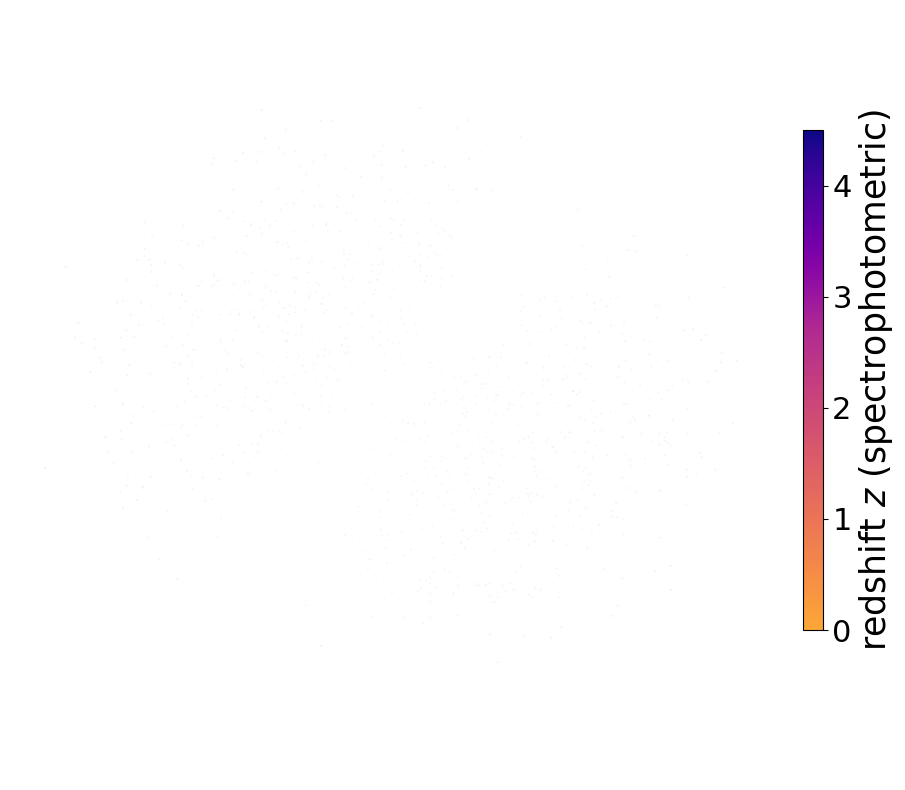
\includegraphics[width=0.48\textwidth]{gcathi_3d.png}}
    \hspace{1em}
    \subfloat[\label{fig:sdss_3d}]{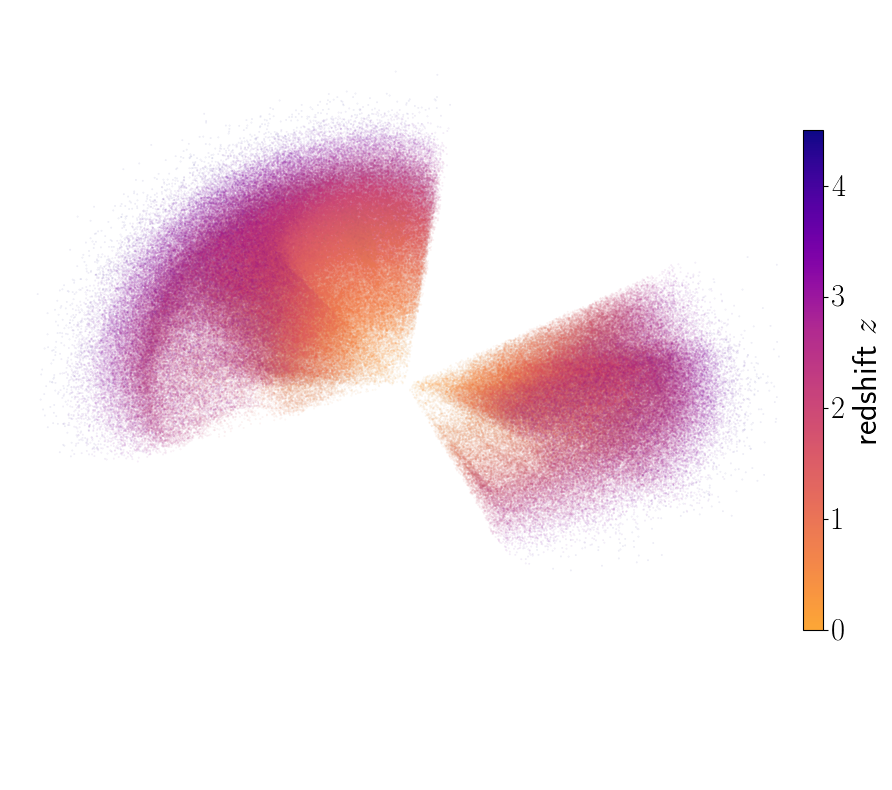
\includegraphics[width=0.48\textwidth]{sdss_3d.png}}

    \caption{(a) A 3D projection of the \catalog. (b) The same projection for the quasars in \SDSS DR16Q. The colorbar shows the redshifts of the quasars ($\zspz$ for \cat, $\zgaia$ for \SDSS). \cat spans a larger volume and has a cleaner selection function than the \SDSS sample. \emph{An animated version is available at} \url{https://cosmo.nyu.edu/ksf/QSOs.gif}.}
    \label{fig:3d}
\end{figure*}

We show a 3D projection of the \cat catalog in Figure~\ref{fig:gcathi_3d}, using our $\zspz$ redshift estimates converted to spatial coordinates with a fiducial Planck cosmology.
Figure~\ref{fig:sdss_3d} shows the \SDSS quasar sample for comparison.
The \catalog spans a much larger volume than \SDSS, and also has a cleaner selection function; the distribution looks homogeneous in 3D, while strong spatial selection effects can be seen in the \SDSS sample.

\begin{figure*}
    \centering
    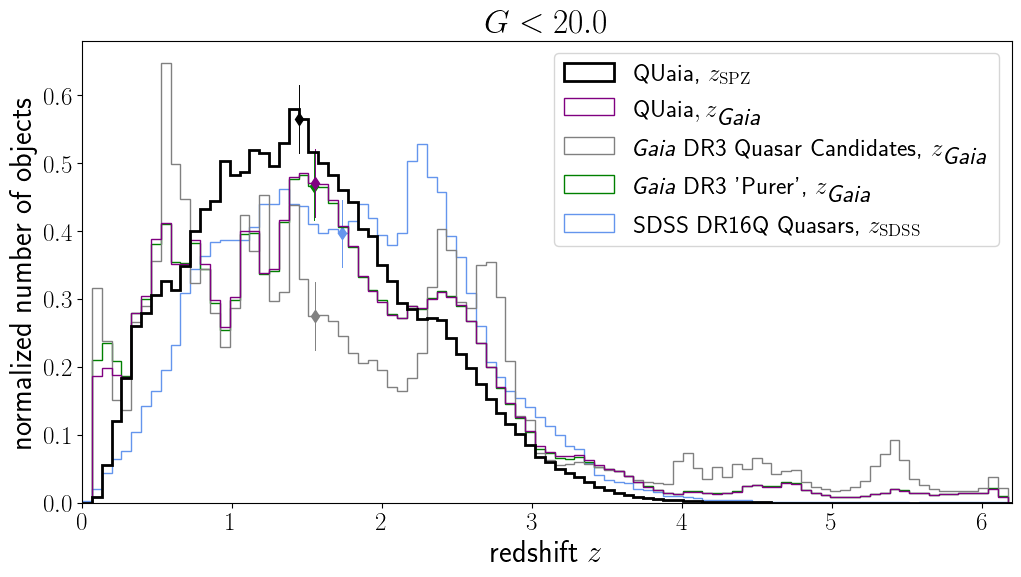
\includegraphics[width=0.9\textwidth]{redshift_dists_Glo.png}
    \caption{Redshift distribution of the $G<\protect\Glo$ \catalog for our spectro-photometric redshift estimates $\zspz$ (black), normalized to the total number of objects. For comparison we also show the normalized distributions of the \Gaia redshift estimates $\zgaia$ for the same \cat sources (purple); $\zgaia$ for the sources in the full \Gaia quasar candidate sample (grey); $\zgaia$ for the \Gaia DR3 ''purer'' subsample (green); and the \SDSS redshifts $\zsdss$ for the \SDSS DR16Q quasar sample (blue). All distributions are shown for $G<\protect\Glo$ subsamples for clear comparison. The median redshift of each distribution is shown by the diamond and vertical line in the respective color.} 
    \label{fig:z_dists}
\end{figure*}

We show the redshift distribution of \cat in Figure~\ref{fig:z_dists}.
The distribution of our \Gaia--\unWISE--\SDSS spectro-photometric redshift estimates, $\zspz$, for the catalog down to $G<\Glo$ is shown in black.
We compare this to other samples cut to the same $G$ limit: the \Gaia redshifts $\zgaia$ for the same sample; $\zgaia$ for the all sources in the \Gaia quasar candidates sample (that have redshift  estimates); $\zgaia$ for sources in the purer \Gaia sample; and $\zsdss$ for the \SDSS DR16Q sources.
We see that the SPZ redshifts have a smoother distribution than the others, with a clear peak around $z=1.5$; the median value is \val{zmed_gcatlo}.
These SPZ estimates have also greatly reduced the high-$z$ tail present in the \Gaia redshifts.
There are still a significant amount of intermediate-$z$ objects; $\val{p_above_zintermediate_gcatlo}\%$ ($N=\val{N_above_zintermediate_gcatlo}$) of the sources in the $G<\Glo$ catalog have $z>\val{zintermediate}$.
We note that the $\zgaia$ redshift distribution for the purer sample is very similar to those same redshift estimates for \cat; this is partially because a very high fraction of the objects in \cat are also in the larger \Gaia purer sample (see Figure~\ref{fig:frac_matrix}).
We also see a slight bump in the $\zspz$ distribution around $z\sim2.25$, the same location as the peak in the \SDSS DR16Q quasar distribution.
This indicates that features in the training sample have been imprinted onto our redshift model, though the distortion is quite slight.

\begin{figure}
    \centering
    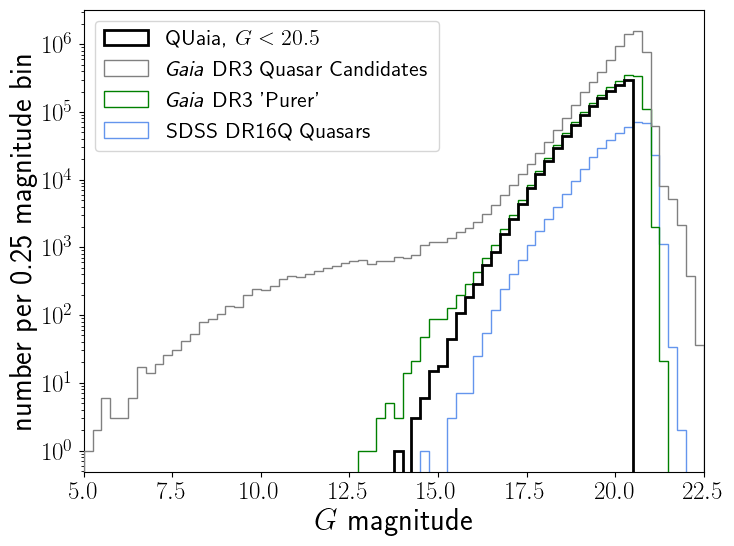
\includegraphics[width=0.6\columnwidth]{G_dist}
    \caption{Distribution of $G$ magnitudes of \cat (black), compared to the full \Gaia candidates sample (grey), the {\Gaia} 'purer' sample (green), and the \SDSS DR16Q quasar sample (blue).}
    \label{fig:G_dist}
\end{figure}

We show the $G$-band magnitude distribution of \cat is shown in Figure~\ref{fig:G_dist}, in comparison the other \Gaia and \SDSS quasar samples described above.
We see that our catalog (as well as the \Gaia 'purer' sample) has removed all of the sources with excessively bright (for quasars) magnitudes $G<12.5$ that are present in the full \Gaia sample, as well as many sources with $12.5<G<16$.
For the \Gaia DR3 and \SDSS samples, the number of quasars drops off sharply after $G\sim20.75$; to avoid the complicated selection effects at these depths, we limit our catalog to $G<\Ghi$ as shown.
We also note that the \SDSS DR16 quasars do not extend as bright as \cat, and this extrapolation past the training set could bias the results in this regime, though in practice this affects very few sources.


\subsection{The selection function model}
\label{sec:selfunc}

\begin{figure}
    \centering
    \subfloat[\label{fig:selection_function_map}]{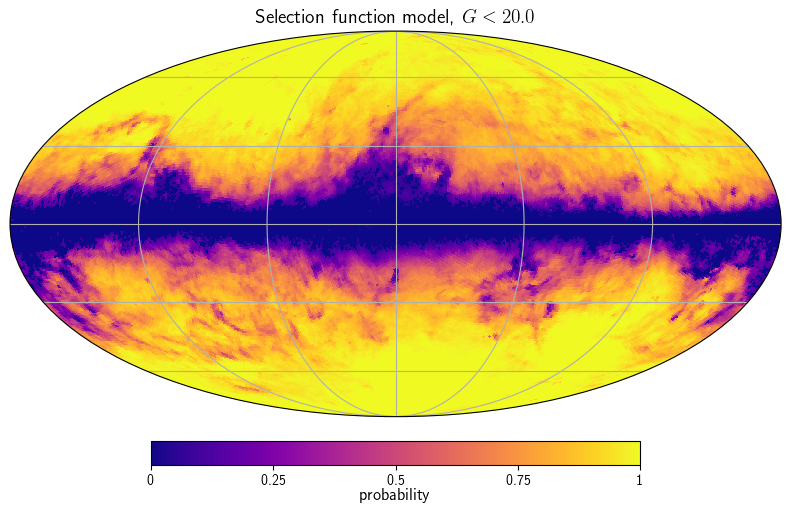
\includegraphics[width=0.75\columnwidth]{selection_function_Glo.png}}
    \vspace{0.1ex}
    \subfloat[\label{fig:selection_function_residuals}]{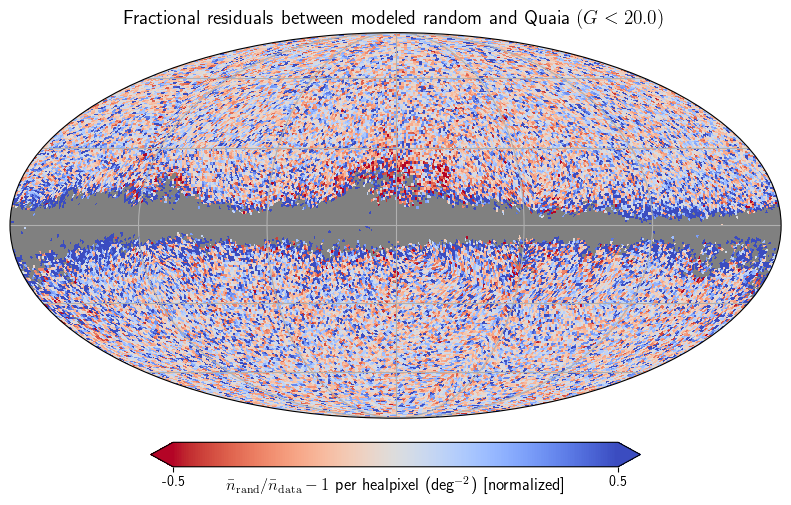
\includegraphics[width=0.75\columnwidth]{residuals_Glo.png}}
    \caption{(a) The selection function map for the $G<\protect\Glo$ \catalog, based on a Gaussian process model of the dust, stellar distribution, and $M_{10}$. (b) The fractional residuals between a random catalog down-sampled by the modeled selection function and the true $G<\protect\Glo$ \catalog.}
    \label{fig:selection_function}
\end{figure}

We show the results of our selection function modeling (\S\ref{sec:selfunc_methods}) for the $G<\Glo$ catalog in Figure~\ref{fig:selection_function}.
The selection function map is shown in Figure~\ref{fig:selection_function_map}: the relationship to the dust and stellar distribution maps is clear visually.
In Figure~\ref{fig:selection_function_residuals}, we show the residuals between a random catalog down-sampled by this selection function and the true quasar catalog.
The residuals generally look like homogenous noise, indicating a good fit; the root mean squared fractional error is \val{rmse_fractional_residuals_Glo}.
Around the edges of the galactic plane the random is over-predicted, meaning the completeness there was predicted to be higher than it actually is; this could indicate that our templates are not fully capturing the selection effects.
This issue could be circumvented by applying a latitude cut for sensitive analyses.
The selection function map for the $G<\Ghi$ catalog (not shown) is also provided as a data product, as well as the code to fit the selection function for any other subsample of the catalog.


\subsection{Comparison to existing quasar catalogs}
\label{sec:comparison}

\begin{figure*}
    \centering

    \subfloat[\label{fig:2d_gpurer_Ghi}]{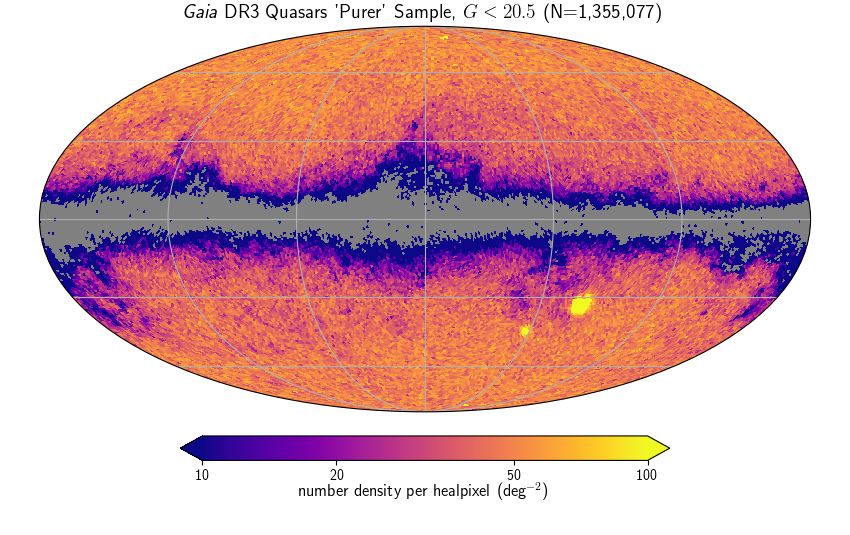
\includegraphics[width=0.45\textwidth]{gpurer_Ghi_2d.png}}
    \hspace{5ex}
    \subfloat[\label{fig:2d_eboss}]{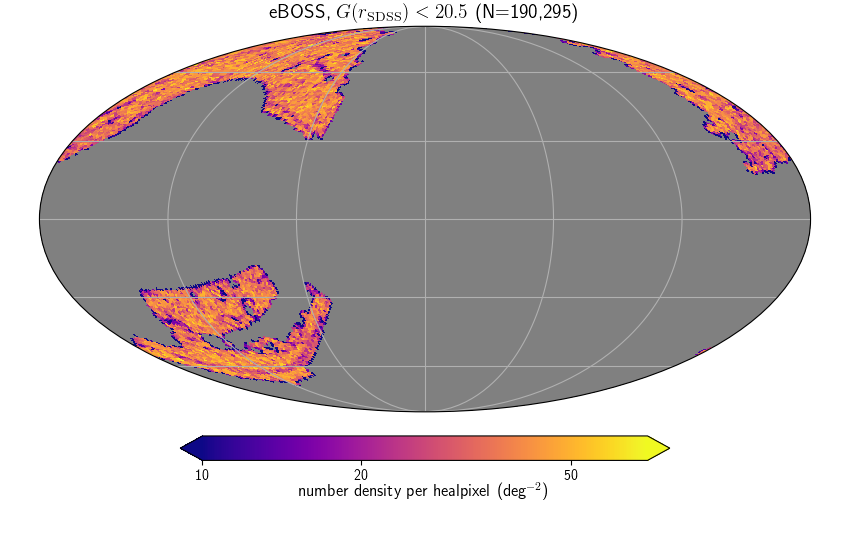
\includegraphics[width=0.45\textwidth]{eboss_Ghi_2d.png}}
    
    \subfloat[\label{fig:2d_wiseps}]{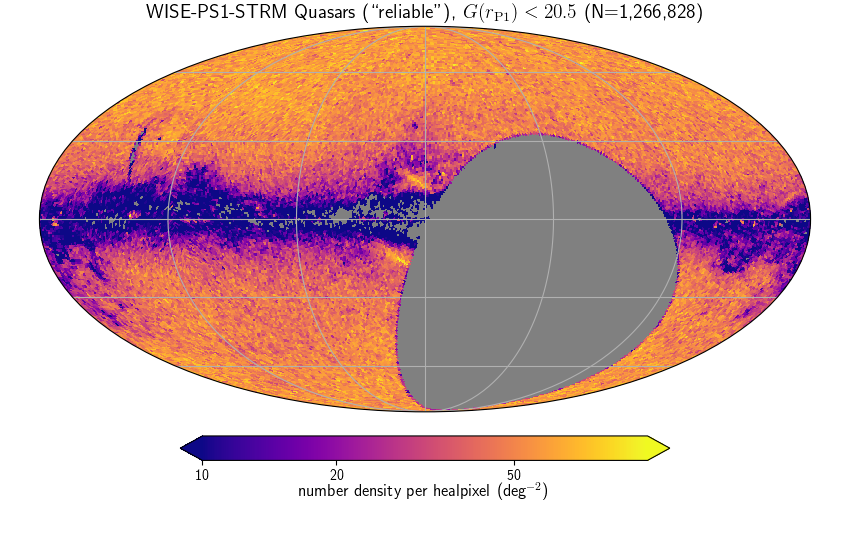
\includegraphics[width=0.45\textwidth]{wiseps_Ghi_2d.png}}
    \hspace{5ex}
    \subfloat[\label{fig:2d_milliquas}]{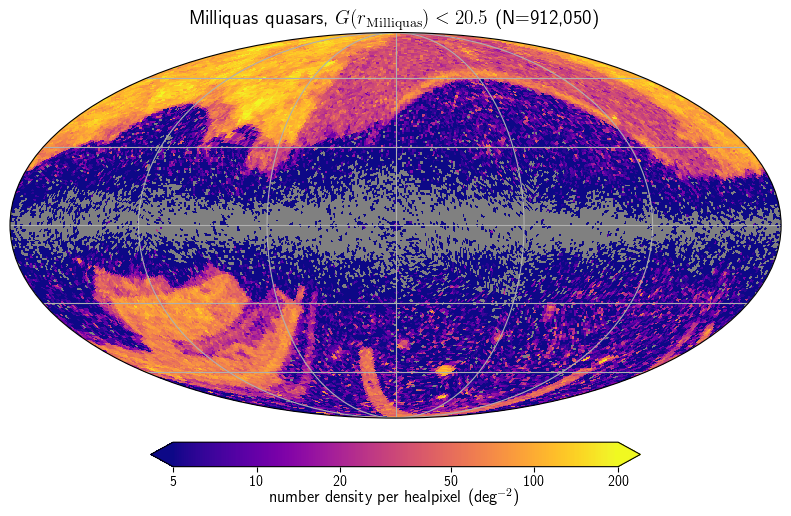
\includegraphics[width=0.45\textwidth]{milliquas_Ghi_2d.png}}

    \caption{Other current quasar catalogs for comparison with our \catalog. All are shown for sources with $G<\protect\Ghi$ or the equivalent converted from another band, in galactic coordinates and displayed using a Mollweide projection. The catalogs are: (a) the \Gaia DR3 'purer' sample, (b) the eBOSS sample, (c) the WISE-PS1-STRM catalog, and (d) the Milliquas catalog. Note that the color bars have different scales in each panel.}
    \label{fig:2d_comp}
\end{figure*}

We compare the \catalog to other existing quasar catalogs: 
Projections of these catalogs are shown in Figure~\ref{fig:2d_comp}. 
We show the \Gaia purer sample (Figure~\ref{fig:2d_gpurer_Ghi}); eBOSS, the current best spectroscopic sample (Figure~\ref{fig:2d_eboss}); a cross-matched catalog of WISE and Pan-STARRS (WISE-PS1), a current leading large-area photometric redshift quasar sample (Figure~\ref{fig:2d_wiseps}); and  Milliquas, a meta-catalog compiling confirmed quasars from the literature (Figure~\ref{fig:2d_milliquas});.

The \Gaia purer sample is described in \S\ref{sec:data_gaia}; here we include only sources with QSOC redshift estimates ($\zgaia$).
The eBOSS catalog is detailed in \cite{ross_completed_2020}; we have included both eBOSS and legacy SDSS quasars and applied the clustering cuts of requiring sectors to have $>0.5$ completeness and redshift success rate, and removed source with \texttt{ZWARNING}!=0.
The WISE-PS1 sample was constructed by \cite{beck_wise-ps1-strm_2022}, based on the Source Types and Redshifts with Machine learning (STRM) algorithm by \cite{beck_ps1-strm_2020}.
The quasar catalog with updated photometric redshifts is presented by \cite{kunsagi-mate_photometric_2022}; here we include only those quasars with redshifts labeled ``reliable'', which is $\val{p_reliable_wiseps}\%$ of the sample.
The Milliquas catalog was compiled by \cite{flesch_million_2021}; a significant portion of the sources are from \SDSS and \textsl{AllWISE}.
For each of these samples, we have shown quasars brighter than a limiting magnitude of $G\sim\Ghi$; for the non-\Gaia catalogs we convert to $G$ from the survey's $r$-band magnitude using the conversion in equation (2) of \cite{proft_exploration_2015}, which is based on the \SDSS $r'$ band.
While this should give a reasonable estimate for the \SDSS sample (using $r_\text{SDSS}$) and the WISE-PS1 sample (using $r_\text{PS1}$ which is very similar to $r_\text{SDSS}$), it may not be as reliable for Milliquas which catalogs ''red'' magnitudes from various sources, as well as for sources with $z>3$ which were not included in the \cite{proft_exploration_2015} fit.

\begin{table*}
    \centering
    \caption{A comparison between \cat and other existing quasar catalogs. All catalogs have been limited to $G<\protect\Ghi$ or the rough equivalent converted from another band, and exclude areas with high dust extinction ($A_v > \protect\val{Avhi}$). We show the number of sources $N$, the fraction of sky area covered $f_\mathrm{sky}$, the mean number density per square degree $\bar{n}$, the spanning volume between $0.8<z<2.2$ $V_\mathrm{span}$, the effective volume $V_\mathrm{eff}$, the median redshift $z_\mathrm{med}$, and the fraction of objects with $|\delta z| \equiv |\dz| < 0.01$ and $<0.1$ (where applicable).}
    \centering
    \input{data/data_quaia/comparison_table.txt}
    \label{tab:comparison}
\end{table*}

A summary of the catalogs is shown in Table~\ref{tab:comparison}, for the $G<\sim$\Ghi subsamples.
(We exclude Milliquas from this comparison as it is so heterogeneous.)
For these quantifications we exclude areas that have $A_v > \val{Avhi}$, as well as healpixels with no quasars.
For the sky fraction $f_\mathrm{sky}$, we see that \cat and \Gaia purer are limited only by the dusty regions, and cover over 30\% more area than WISE-PS1 (which is limited by Pan-STARRS), and nearly $6\times$ that of eBOSS.
Compared to the \Gaia purer sample, the \catalog has a slightly smaller number of sources, but due to its redshift distribution gives a slightly higher effective volume.
The on-sky number density is similar for all of the catalogs, with WISE-PS slightly higher as it has a similar number of objects to the \Gaia catalogs but over a smaller area.

For the volume comparison, we compute two different volumes. 
The first is a simple ``spanning'' volume, $V_\mathrm{span}$, which is just the comoving volume in the sky area of the survey (as given by $f_\mathrm{sky}$ of the full sky area) in a redshift range $0.8<z<2.2$, a typical redshift rangle for clustering analyses (taken from the range of the eBOSS ``clustering'' sample).
Thus it compares in the same way as the survey areas, but gives an idea of the physical volume the catalogs span.
The second is the effective volume $V_\mathrm{eff}$, which depends on the number density as a function of redshift and the power spectrum value $P(k)$, integrated over the physical volume.
We use the same $P(k)$ for all catalogs, $4 \times 10^4 (\hMpc)^3$, based on the value for the eBOSS quasars at around $k \sim 0.01$ \citep{mueller_clustering_2021}.
We see that the effective volume of \cat is surpassed only slightly by WISE-PS1, and is over $6 \times$ that of eBOSS. 

The catalogs all have a similar median redshift, around $1.4 < z < 1.6$.
% $\val{p_acc_zspz_dzhi_Glo}\%$
However, they have significantly different redshift precision; in Table~\ref{tab:comparison} we show comparisons to spectroscopic redshifts for the catalogs to which this is applicable.
We see that both of the \Gaia catalogs have a similar fraction of high-precision redshifts ($|\dz| < 0.01$), but \cat has a much higher fraction of redshifts that are not bad outliers ($|\dz| < 0.1$) compared to \Gaia purer.
WISE-PS1 falls between the two in terms of bad outliers, but has an extremely low fraction of high-precision redshifts as it is a photometric survey.
The eBOSS sample has spectroscopic redshifts, so these are almost all very high-precision; \cite{lyke_sloan_2020} calculated that less than 1\% of the SDSS DR16Q redshifts are outliers with $v < 3000\,\text{km s}^{-1}$ ($|\dz| > 0.01$); note that this is a slightly different sample than the eBOSS quasars, but we can expect it to be similar.

We also note that the ongoing DESI survey \citep{Aghamousa2016} will observe a high density of quasars over a large sky area \citep{yeche_preliminary_2020}, which will be competitive with and complementary to this \Gaia--\unWISE catalog.


\subsection{Catalog format}
\label{sec:format}

\begin{table*}
    \caption{The format and column descriptions of the \catalog, published as a FITS data file. For the example entry, we show the first catalog row that has values for all of the columns.}
    \centering
    \input{data/data_quaia/catalog_table.txt}
    \label{tab:catalog}
\end{table*}

The \catalog contains our decontaminated quasar sample with computed redshift information, relevant \Gaia properties, and cross-matched catalog information.
The complete catalog format with column names, units, column descriptions, and an example entry, are shown in Table~\ref{tab:catalog}.
Additional information for the sources can be obtained by joining the catalog with the relevant data source with the associated identifier (\Gaia or \unWISE).
We include only sources with $G<\Ghi$ in the catalog; we also publish a version limited to $G<\Glo$, along with the selection function models fit to each (\S\ref{sec:selfunc}) and ''random'' catalogs generated from the selection functions.
The catalog includes our SPZ redshifts $\zgaia$ along with redshift errors $\sigma_{z\mathrm{SPZ}}$, sky position, \Gaia photometry, \unWISE photometry, and proper motion information.
The catalog is in FITS format, and units and descriptions are provided for each column.
% For quasars in our catalog that have an \SDSS match, we include the \SDSS source ID and the \SDSS spectroscopic redshift.
% We also include a flag for whether the quasar was included in the \Gaia purer sample.


\subsection{Potential applications}
\label{sec:applications}

The \catalog has many potential applications.
The immense volume of quasars, which are highly biased cosmic web tracers, lends itself to large-scale structure analyses.
It is particularly well-suited to cross-correlations with other all-sky observations, such as cosmic microwave background lensing to constrain cosmological parameters and primordial non-Gaussianity (Fabbian et al., in prep.); as a 2D measurement, this is conveniently less sensitive to redshift errors. 
Cross-correlations with photometric galaxy surveys could be used to measure infer quasar environments and measure the baryon acoustic feature; the 3-d quasar auto-correlation may also contain useful cosmological information.
The catalog is perhaps the best current sample for testing homogeneity or measuring a potential dipole (Hogg et al., in prep.).

The catalog is also well-suited for void studies, including constraining core cosmological parameters with the void size distribution (Arsenov et al., in prep.).
Another measurement enabled by the catalog is the cross-correlation of quasar proper motions with the large-scale structure, which gives a direct estimate of the cosmological quantity $f \sigma_8 H_0$ (Duncan et al., in prep.).
The catalog is additionally useful for astrophysical analyses of quasar properties, given its large sky coverage and multi-band photometry.


\section{Summary \& Data Access}
\label{sec:summary}

We have constructed a new quasar catalog, the \catalog (\cat), designed for cosmological studies, derived from the \Gaia DR3 quasar candidates sample and using \unWISE photometry.
Our key contributions and the features of the catalog are as follows:
\begin{itemize}
\setlength\itemsep{0.5ex}
    \item We have decontaminated the \Gaia DR3 quasar candidates sample with proper motion cuts and optimized color cuts based on \Gaia and \unWISE photometry. This reduced the number of known contaminants by \val{factor_reduction_contaminants} while only excluding $\val{p_sqall_excluded_clean}\%$ of known quasars with respect to the superset of \Gaia quasar candidates (that have \unWISE photometry, \Gaia redshifts, and a $G$-magnitude cut of $G<\Gmax$).  
    %% ACE: add how much the purity improved here.
    \item The catalog extends to a limiting magnitude of $G<\Ghi$ and contains \val{N_gcathi} sources; we also release a brighter, cleaner sample limited to $G<\Glo$, which has \val{N_gcatlo} sources.
    \item \cat covers the entire sky, only limited by selection effects near the galactic plane; excluding highly dust-extincted regions ($A_v > \val{Avhi}$), this results in an area of \val{area_below_Avhi} ($f_\mathrm{sky}=\val{fsky_below_Avhi}$).
    \item We have improved the \Gaia redshift estimates using a \knn model trained on these redshifts and \Gaia and \unWISE colors with \SDSS spectroscopic redshift labels, producing spectro-photometric redshifts. The median redshift of the $G<\Glo$ catalog is $z_\mathrm{med}=\val{z_med_gcatlo}$, with $\val{p_acc_zspz_dzhi_Glo}\%$ ($\val{p_acc_zspz_dzlo_Glo}\%$) of redshifts within $|\dz|<\val{dzhi}$ (\val{dzlo}) of \SDSS redshifts. This is a reduction in the number of catastrophic outliers by \val{factor_reduction_outliers_dzhi_Glo} (\val{factor_reduction_outliers_dzmid_Glo}) compared to the \Gaia redshift estimates.
    \item We produced a data-driven model of the selection function which includes the systematic effects of dust, stars, and the \Gaia scanning law. We used this to generate random catalogs of Poisson-distributed points with the same selection effects as \cat.
\end{itemize}

The catalog and related data products will be publicly available, along with documentation.
The code used to generate this catalog is open-source and available at \url{https://github.com/kstoreyf/gaia-quasars-lss}.

\textit{Software:} Astropy \citep{the_astropy_collaboration_astropy_2013, the_astropy_collaboration_astropy_2018, the_astropy_collaboration_astropy_2022}, numpy \citep{VanDerWalt2011}, IPython \citep{Perez2007}, scipy \citep{Virtanen2020}, matplotlib \citep{Hunter2007}, healpy \citep{gorski_healpix_2005, zonca_healpy_2019}, george \citep{Ambikasaran2016}

\section{Chapter acknowledgments}

The authors are grateful to the \Gaia collaboration members, in particular Coryn Bailer-Jones, Morgan Fouesneau, Anthony Brown, Ludovic Delchambre, Tristan Cantat-Gaudin, and Arvind Hughes.
The authors also thank Giulio Fabbian, Nestor Arsenov, Andras Kovacs, Michael Blanton, An\v{z}e Slosar, David Alonso, Iain Duncan, Lyuba Slavcheva-Mihova, Alex Malz, Lehmann Garrison, and Mehdi Rezaie for helpful discussions.
Additionally, the authors thank the attendees of the \Gaia F\^{e}te and the members of the Astronomical Data group at the Center for Computational Astrophysics for useful feedback.
This work has made use of data from the European Space Agency (ESA) mission {\it Gaia} (\url{https://www.cosmos.esa.int/gaia}), processed by the {\it Gaia} Data Processing and Analysis Consortium (DPAC, \url{https://www.cosmos.esa.int/web/gaia/dpac/consortium}). 
Funding for the DPAC has been provided by national institutions, in particular the institutions participating in the {\it Gaia} Multilateral Agreement.
K.S.F. is supported by the NASA FINESST program under award number 80NSSC20K1545.
This research made use of computational resources at New York University; the authors thank the NYU high-performance computing team.

